%% ----------------------------------------------------------------
%% Thesis.tex -- MAIN FILE (the one that you compile with LaTeX)
%% ---------------------------------------------------------------- 

% Set up the document
\documentclass[a4paper, 12pt, oneside]{sproj_report}  % Use the "Thesis" style, based on the ECS Thesis style by Steve Gunn
\graphicspath{{Figures/}}  % Location of the graphics files (set up for graphics to be in PDF format)

% Include any extra LaTeX packages required
\usepackage[square, numbers, comma, sort&compress]{natbib}  % Use the "Natbib" style for the references in the Bibliography

\usepackage{verbatim}  % Needed for the "comment" environment to make LaTeX comments
\usepackage{multirow} % for psnr and ssim tables
\usepackage{booktabs} % for psnr and ssim tables
\usepackage{svg} % for svg images

% \usepackage{vector}  % Allows "\bvec{}" and "\buvec{}" for "blackboard" style bold vectors in maths

\usepackage{url}
\usepackage{natbib}
\usepackage{fancyhdr}
\usepackage{amsmath}
\usepackage{algorithm}
\usepackage{algpseudocode}
%\usepackage{subfig}
\hypersetup{urlcolor=blue, colorlinks=true}  % Colours hyperlinks in blue, but this can be distracting if there are many links.

% remove the unnecessary spacing before and after the headings/subheadings
\usepackage[compact]{titlesec}
\titlespacing{\section}{0pt}{*0}{*0}
\titlespacing{\subsection}{0pt}{*0}{*0}
\titlespacing{\subsubsection}{0pt}{*0}{*0}

\setlength{\parskip}{6pt}
%\setlength{\parsep}{0pt}
%\setlength{\headsep}{0pt}
%\setlength{\topskip}{0pt}

\thispagestyle{fancy}
\fancyhead{}
\fancyfoot{}
\lfoot{Unrolled Optimization and Matrix Completion}
\rfoot{\arabic{page}}
\renewcommand{\headrulewidth}{0pt}
\renewcommand{\footrulewidth}{0.4pt}
%% ----------------------------------------------------------------
\begin{document}
\frontmatter	  % Begin Roman style (i, ii, iii, iv...) page numbering

% Set up the Title Page
\title  {Unrolled Optimization and Matrix Completion}
\degree{BS Mathematics-Economics}
\session {2023 - 24}
\advisor {Dr. Muhammad Tahir, \\Associate Professor, EE}
\coadvisor{Dr. Adnan Khan, \\ Associate Professor, MATHS}
%authors should be written in the cls file
\addresses  {\deptname \\ \univname}  % Do not change this here, instead these must be set in the "Thesis.cls" file, please look through it instead
\date       {\today}
\subject    {}
\keywords   {}

\maketitle
\clearpage
%% ----------------------------------------------------------------
% The Abstract Page
\addtotoc{Abstract}  % Add the "Abstract" page entry to the Contents
\abstract{
%\addtocontents{toc}{\vspace{1em}}  % Add a gap in the Contents, for aesthetics

In this report, we deal with the problem of matrix completion using the recently introduced technique of deep unfolding. Matrix completion is an old yet important problem in signal processing and compressed sensing and numerous methods have been proposed to solve it, but deep unfolding has shown immense promise and has been able to solve this problem with unprecedented accuracy and speed. Despite this, the research in applying this technique to matrix completion algorithms, especially those that utilize the matrix factorization approach, which has been the bulk of recent algorithms in this field, has been scant. Our research is an attempt to boost interest in this specific application of deep unfolding, as we introduce two new deep-unfolded models, ConvMC-Net and ConvHuberMC-Net. They respective utilize the unfolded versions of augmented Lagrange multipliers (ALM) and M-estimation, which, in turn, is an application of Huber regression. We provide a thorough comparison of more than a dozen algorithms proposed in the near past and investigate their performances on multiple tasks, using multiple shapes, and conclude with the algorithms that seem to perform best (in terms of inference time and accuracy) and the potential for further improvement in the algorithms that we propose.

Code for ConvMC-Net and ADMM-Net, M-estimation, and ConvHuberMC-Net is provided on the following three GitHub repositories:

- \url{https://github.com/Talha-Nehal-Undegrad-Study/convmc-net} \\
- \url{https://github.com/Talha-Nehal-Undegrad-Study/M-estimation-RMC} \\
- \url{https://github.com/Talha-Nehal-Undegrad-Study/ConvHuberMC-Net}}

\clearpage  % Abstract ended, start a new page

%% ----------------------------------------------------------------

\setstretch{1.3}  % Reset the line-spacing to 1.3 for body text (if it has changed)

% The Acknowledgements page, for thanking everyone
\acknowledgements{
%\addtocontents{toc}{\vspace{1em}}  % Add a gap in the Contents, for aesthetics

The authors wish to express sincere appreciation to Dr. Muhammad Tahir and Dr. Adnan Khan for their dedicated supervision during the course of this senior year project and in the preparation of this manuscript. 

}
\clearpage  % End of the Acknowledgements

%% ----------------------------------------------------------------
% Declaration Page required for the Thesis, your institution may give you a different text to place here
\Declaration{
%\addtocontents{toc}{\vspace{1em}}  % Add a gap in the Contents, for aesthetics

“We the undersigned, certify that this submission is the original work of members of the group and meets the Faculty\textsc{\char13}s Expectations of Originality":

\bigskip
\begin{enumerate}
\item Talha Ahmed [2024-10-0033] \\ Signed:~~ \rule[0em]{10em}{1.0pt} 24100033@lums.edu.pk \\ \\
\item Nehal Ahmed Shaikh [2024-02-0001]\\ Signed:~~ \rule[0em]{10em}{1.0pt} 24020001@lums.edu.pk \\ \\
\end{enumerate}

\large{\textbf{Advisor}}\\
\large{\textbf{Dr. Muhammad Tahir}}\\
\rule[0em]{15em}{1.0pt}\\
tahir@lums.edu.pk\\ \\
\large{\textbf{Co-Advisor(s)}}\\
\large{\textbf{Dr. Adnan Khan}}\\
\rule[0em]{15em}{1.0pt}\\
adnan.khan@lums.edu.pk
}
\clearpage     % Declaration ended, now start a new page
%% ----------------------------------------------------------------
\lhead{\emph{Contents}}  % Set the left side page header to "Contents"
\tableofcontents  % Write out the Table of Contents

%% ----------------------------------------------------------------
\lhead{\emph{List of Figures}}  % Set the left side page header to "List if Figures"
\listoffigures  % Write out the List of Figures

%% ----------------------------------------------------------------
\lhead{\emph{List of Tables}}  % Set the left side page header to "List of Tables"
\listoftables  % Write out the List of Tables

%% ----------------------------------------------------------------
\mainmatter	  % Begin normal, numeric (1,2,3...) page numbering
\pagestyle{fancy}  % Return the page headers back to the "fancy" style
\onehalfspacing
% Include the chapters of the thesis, as separate files
% Just uncomment the lines as you write the chapters

\chapter{Introduction} % Write in your own chapter title
\label{Chapter1}
\lhead{} % Write in your own chapter title to set the page header

\section{Motivation}
% Motivate Deep Unfolding and Matrix Completion and in the end link the two. 
Deep unfolding is a recent approach that economizes on data and computational requirements yet solves optimization problems with impressive accuracy. This approach has an important advantage over traditional iterative algorithms in that it is more robust to perturbations in inputs and numerical errors. It also has one over traditional neural networks in that it has significantly lower data and computational requirements to perform reasonably. Matrix completion is a problem where a data set is missing some entries while the non-missing entries are possibly affected by noise. There are various iterative algorithms to solve this problem, but research employing unfolded algorithms has been scant.

\section{Problem Statement}
% Getting benefits of unrolling iterative algorithms to improve inference time and accuracy on datasets corrupted by impulsive GMM noise. 
Our objective is to reap the benefits of unfolded optimization algorithms, namely, faster inferences and higher accuracy scores, on data that has been corrupted by impulsive GMM noise.

\section{General Block Diagram}
% Provide high level diagram of convmc and hubermc and explain the pipeline. i.e. very concisely and briefly mention the matrix factorization vs the PCP formulation on which both are based
ConvMC-Net takes a single zero matrix as input with the goal to process it in a way that brings it as close to the original matrix as possible. The processing basically involves singular value thresholding (SVT), measurement matrices, and algebraic manipulation to create an update equation for a multi-layer neural network that finally outputs the recovered matrix.

ConvHuberMC-Net (shown in Figure \ref{fig:convhubermc_block}), on the other hand, follows a different approach. The model takes the corrupted matrix, perhaps some sensor data, as input, along with two other smaller matrices whose product has the same dimensions as the corrupted matrix. The smaller matrices are then processed via the Huber regression algorithm in each layer of the neural network, potentially being refined in a way that makes their product, the recovered matrix, reasonably similar to the pristine version of the corrupted matrix. Details for both ConvMC-Net and ConvHuberMC-Net in chapter 3. 

\begin{figure}
    \centering
    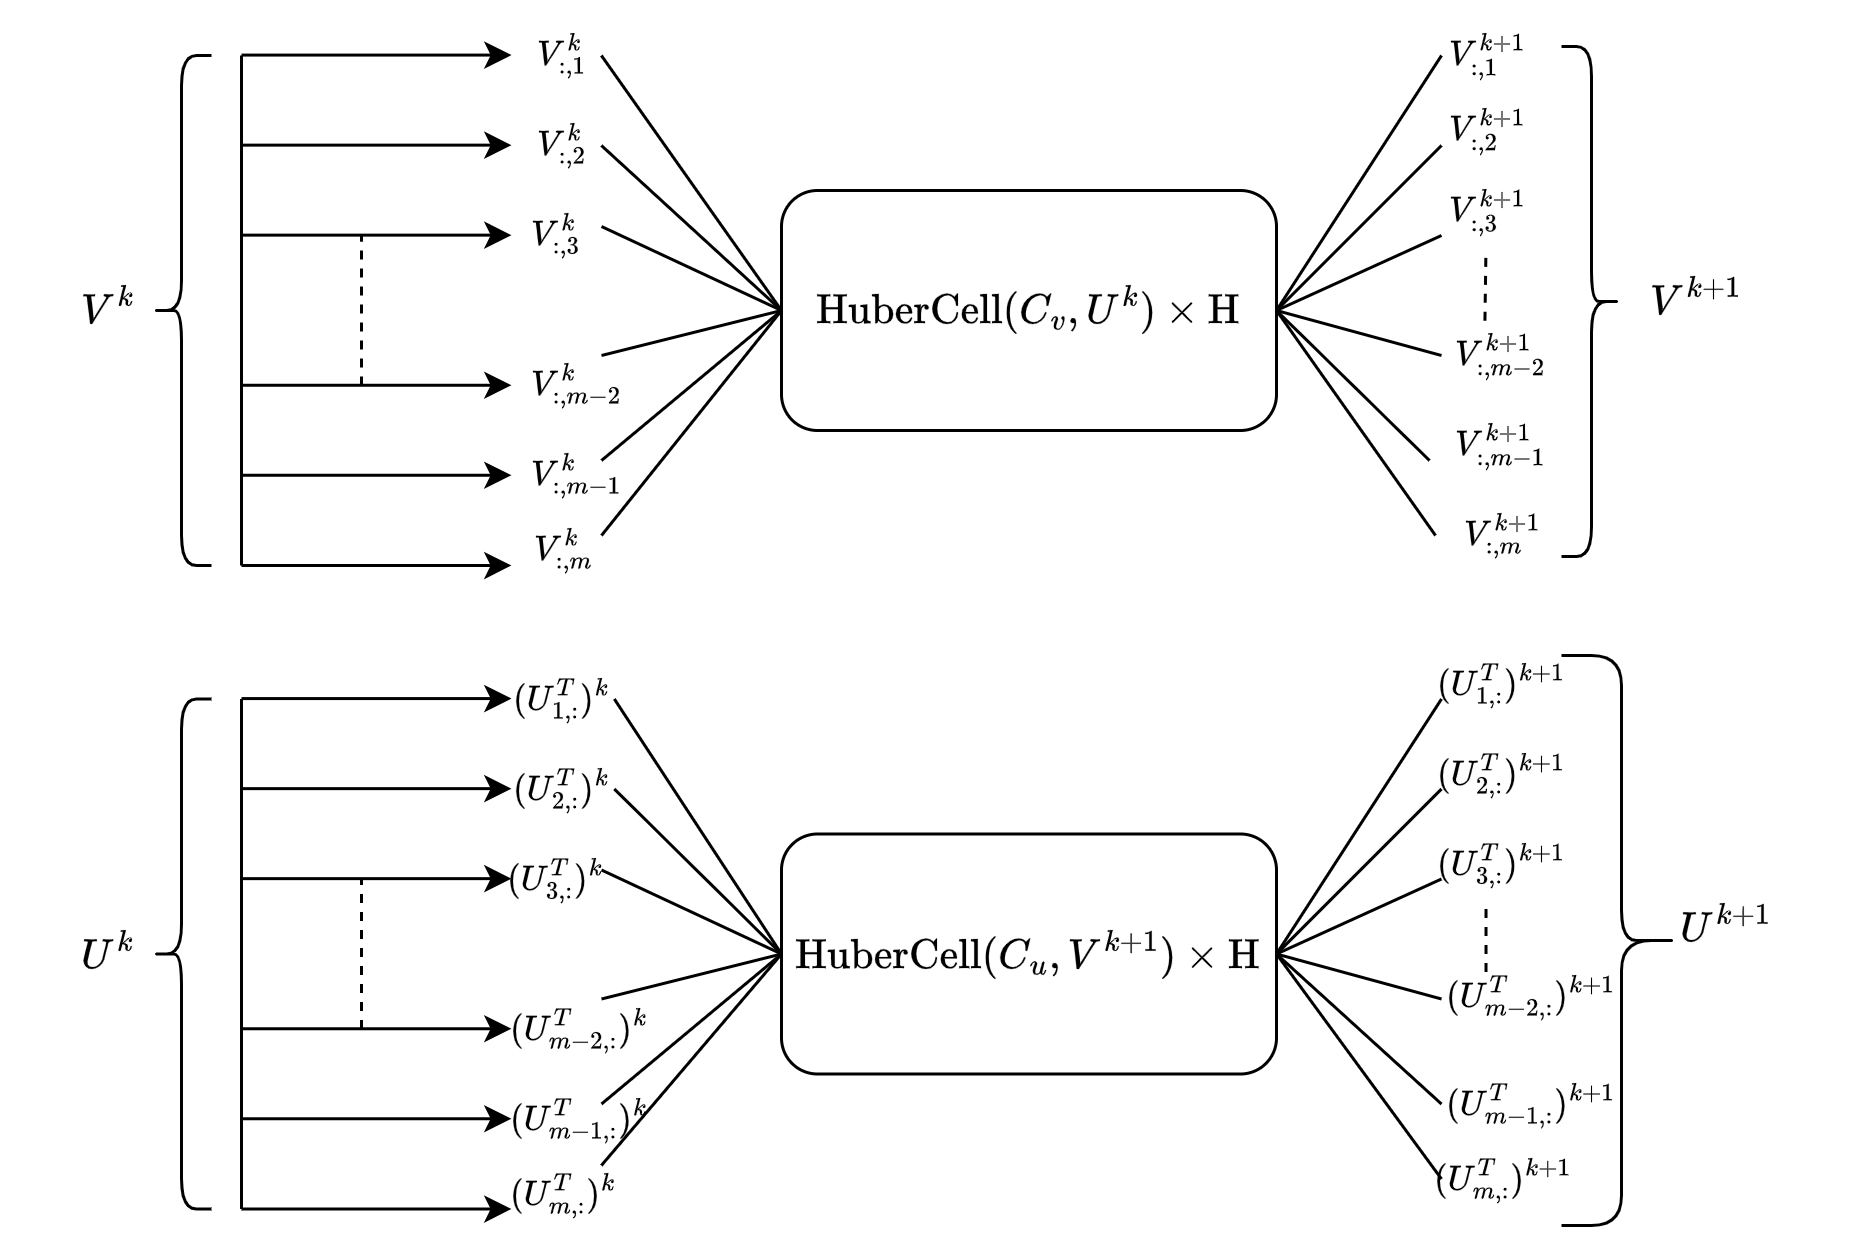
\includegraphics[scale=0.25]{HuberMC-Net}
    \caption{Block diagram of ConvHuberMC-Net}
    \label{fig:convhubermc_block}
\end{figure}

\section{Objectives}
The road map for developing the ideas proposed in this thesis consists of the following sequential objectives:
\begin{enumerate}
    \item Foundational knowledge regarding optimization and matrix completion from \cite{Wright-Ma-2022}.
    \item Identification of data sets related to this task, such as those of sensor networks or grayscale images.
    \item Review of other work done in the domains of matrix completion, compressed sensing, or deep unfolding (e.g., image generation using labelled segmentation maps).
    \item Design and implementation of a pipeline to help achieve our objectives.
\end{enumerate}

\section{Outcomes}
A desirable outcome of this research project is a proven capability to get seamless and accurate image reconstruction or wireless network node measurements or recommendation systems based on supervised methods. As far as social outcomes are considered, we hope that the ideas developed can be used relevant organizations for more accurate decision making.

\section{Outputs}
We intend to deliver a unfolded deep learning architecture that could be used for solving matrix completion problems in Pakistan and elsewhere. This may be presented as an open-source software or as a theoretical framework in a poster, thesis, or research paper.

\section{Timelines and the distribution of work}
% borrow content from compiled report shared with Sir before. 
% Expected:
% 1) Coursework and Preliminary Studies
% 2) Research and Experimentation and Replicating Results
% 3) Refining Shoaib Bhai's work (maybe add footnote here of the slump we faced during this time)
% 4) Literature Review
% 4) Experimenting and Comparing results with different algorithms on different datasets. 
% 5) Further refining pipeline until satisfactory results in most areas
% 6) Finalization
% Reality: 
% 4) Ideation
% 5) Literature Review
% 6) Detailed Experimentation on HuberMC
% 7) Finalization of Deliverables
We originally began this project in June 2023, starting off with an in-depth study of deep learning and signal processing. Eventually, we moved on to studying the work of Shoaib Imran (such as \cite{duparpca} and \cite{dustrpca}), including an incomplete paper and companion code on unfolding the augmented Lagrange multiplier (ALM) for matrix completion. This was the ConvMC-Net model. Our first actual task was to refine and complete the code, run experiments on synthetic and image data sets, compile the results, and compare them with those of existing matrix completion algorithms. Once this was done, the second task was to keep repeating this process until we had satisfactory performance over the two kinds of data sets. The final task was to document this improved performance in a research paper. However, only after we had compiled the results did we realize that our model makes a simplifying assumption: it assumes that the input matrix only has missing entries and is untouched by any kind of noise. Though this is a useful problem to solve in certain scenarios, it is quite limited in its capabilities compared to a model that can also deal with noise. At this point, we delved into the literature to see whether the assumption of noise can be incorporated into ALM and if not, then whether there exist other algorithms that can be unfolded for this task. We eventually settled on M-estimation, which led to our second model, ConvHuberMC-Net. From this point onward, we experimented extensively on several aspects of the new model and concluded with the results presented in this report. 

% \begin{figure}
%   \centering
%   \includegraphics{}
%   \caption{Timeline of the work}
%   \label{fig:timeline}
% \end{figure} % Introduction 

% Chapter 2


\chapter{Background} % Write in your own chapter title
\label{Chapter2}
\lhead{} % Write in your own chapter title to set the page header

\section{Interpretability in AI}

\subsection{Definition}

Over the past decade, the field of artificial intelligence (AI) has experienced rapid growth, becoming increasingly prevalent in automated decision-making processes across various sectors, both public and private. With the proliferation of machine learning systems, there is a growing need to understand and interpret the reasoning behind their decisions.

Interpretability in AI refers to the ability to understand and explain how machine learning models arrive at their conclusions \cite{intepretai}. As machine learning systems become more complex, understanding their decision-making processes becomes increasingly challenging. This lack of interpretability presents a fundamental obstacle to the widespread adoption of AI systems in critical domains.

The discussion surrounding the explainability of AI revolves around the study of how to comprehend the decisions made by machine learning systems and how to design systems whose decisions can be easily understood or interpreted. Strengthening interpretability, verifying the functionality of AI systems, and offering explanations for unexpected behaviors collectively builds trust and confidence in decision-making processes driven by AI.

\subsection{Importance of Interpretability}

In many aspects of society, there exists a fundamental expectation for the right to request an explanation for decisions, particularly when those decisions may have adverse consequences. This expectation extends across various domains, from employment discrimination cases to financial transactions and even military proceedings.

However, when decisions are made by machine learning systems, this expectation becomes more complex. Unlike human decision-makers, machine learning systems may lack the ability to provide explanations for their decisions, posing challenges in ensuring accountability and adherence to established standards.

For modern machine learning systems to integrate safely into existing institutions, especially in high-stakes settings, interpretability becomes essential.  In high-stakes applications such as automated credit scoring, medical diagnoses, hiring, and autonomous driving, the decisions made by these systems can have significant implications for individuals and society at large. Human operators must be able to understand and interpret the decisions made by these systems, allowing for accountability and trust in their outcomes.

In below subsections we discuss the problem of intepretability of AI in \textit{Computer Vision} (CV) and what are some methods used to address it along what are their limitations. 


\subsection{Interpretability in Computer Vision and Saliency Maps}

Interpretability in CV can refer to the ability to explain and understand how a model arrives at its predictions, especially in complex tasks such as image classification.

One popular approach to enhance interpretability in computer vision is the use of saliency maps \cite{saliency}. These maps visualize which areas of an image contribute most to a model's classification decision. For example, when analyzing an image of a German Shepherd classified as a dog, a saliency map may highlight features characteristic of dogs, such as a large muzzle, tail etc.

Figure \ref{fig: saliency_map} below illustrates examples of images alongside their corresponding saliency maps, demonstrating how saliency maps can provide insights into the decision-making process of machine learning models. 

\begin{figure}[htbp]
  \centering
  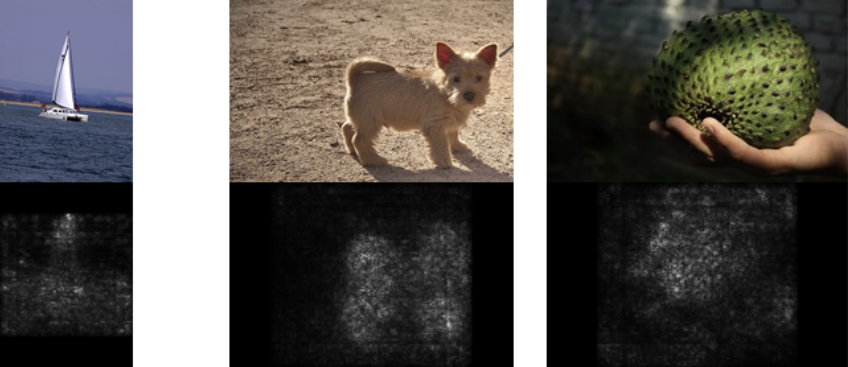
\includegraphics[width=\textwidth]{./Figures/saliency.png}
  \caption{Examples of images and their corresponding saliency maps indicating which parts of the images contribute most to how a machine learning system trained on a large set of images would classify them. Source: \cite{simonyan2014deep}}
  \label{fig: saliency_map}
\end{figure}

\subsection{Visualizing Model Components}

Another effective method for enhancing interpretability is to visualize how different components of a model relate to high-level concepts. For instance, in image classifiers, visualizations can show how different layers of the network detect lines, textures, and objects of increasing complexity.

Figure \ref{fig: layer_perspective} showcases examples of visualizations depicting what different layers of an image classification network "see," highlighting the progression from simple features to more complex objects.

\begin{figure}[htbp]
  \centering
  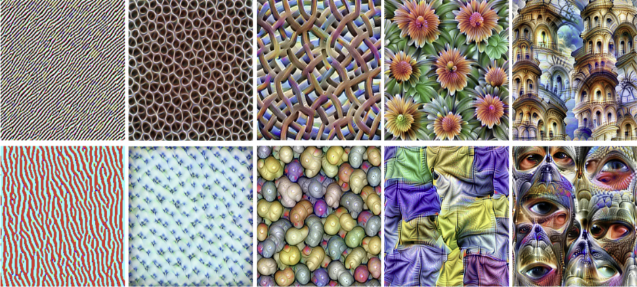
\includegraphics[width=\textwidth]{./Figures/layer_perspective.png}
  \caption{A visualization showing examples of what different layers of an image classification network “see.” The left-most column, depicting an early layer, is picking up lines; middle layers are detecting textures and patterns of increasing complexity; later layers, shown on the right, are looking for objects. Source: \cite{olah2017feature}}
  \label{fig: layer_perspective}
\end{figure}

\subsection{Limitations of Existing Methods}

Despite the effectiveness of saliency maps and visualizations, existing methods for enhancing interpretability have limitations. They often provide only a partial view of the system's decision-making process, lacking a comprehensive understanding of how data and learning algorithms interact during training. As a result, insights obtained from existing methods may be incomplete or require human supervision.


\section{Data-Driven Deep Learning and Model-Based Algorithms}
In the previous section, we discussed the limitations of current methods for achieving interpretability in AI systems. We explored the challenges posed by the increasing complexity of machine learning models and the difficulty in understanding how they reach conclusions. It turns out that to understand why this problem is prevalent, more so now than ever before, lies in the understanding of how traditionally problems in fields like signal processing, digital communications, and medical imaging etc were handled - termed as \textit{Model-Based} methods - vs the more popular approach \textit{Data-Driven} methods. We will explain the key differences between these two using a nice example found in \cite{LUIJTEN2023677}. 

\subsection{Model-Based Methods}

Consider the following general linear model:

\begin{equation}
    \mathbf{y} = \mathbf{A}\mathbf{x} + \mathbf{n} \label{eq:1}
\end{equation}

In this model:
\begin{itemize}
    \item $\mathbf{y}$ represents the observed signal or image, possibly corrupted by noise during acquisition or transmission.
    \item $\mathbf{A}$ is the measurement or feature matrix.
    \item $\mathbf{x}$ denotes the signal of interest (e.g., the clean or original image).
    \item $\mathbf{n}$ is the noise vector, which could result from sensor noise, environmental factors, or compression artifacts.
\end{itemize}

In many signal processing problems, including image denoising, this linear model serves as a basis \cite{elad2023image}.

Sometimes, the noise vector comprises a combination of sparse, high-variance components and dense, low-variance Gaussian noise, known as impulsive Gaussian Mixture Model (GMM) distributed noise (reference needed). We'll delve into this further when discussing matrix completion.

Our objective is to recover the clean or original image as accurately as possible.

By applying Bayes’ rule, we define the posterior probability of $\mathbf{x}$ given $\mathbf{y}$ as the product of the likelihood $p(\mathbf{y|x})$ and a prior $p(\mathbf{x})$, yielding:

\begin{equation}
    p(\mathbf{x|y}) = \frac{p(\mathbf{y|x})p(\mathbf{x})}{p(\mathbf{y})} \label{eq:2}
\end{equation}

From Equation~\eqref{eq:2}, a maximum a posteriori (MAP) estimator for Equation~\eqref{eq:1} is derived:

\begin{equation}
    \hat{\mathbf{x}}_{\text{MAP}} = \arg\max_{\mathbf{x}} p(\mathbf{x|y}) = \arg\max_{\mathbf{x}} p(\mathbf{y|x})p(\mathbf{x}) \label{eq:4}
\end{equation}

This estimator provides the most likely estimate according to the posterior distribution. Assuming an additive Gaussian white noise vector $\mathbf{n}$ in Equation~\eqref{eq:1}, i.e., $\mathbf{y} \sim \mathcal{N}(\mathbf{Ax}|\sigma^2_n\mathbf{I})$, the MAP estimator can be expressed as:

\begin{equation}
    \hat{\mathbf{x}} = \arg\min_{\mathbf{x}} \|\mathbf{y} - \mathbf{Ax}\|_2^2 + \lambda \log p(\mathbf{x}) \label{eq:5}
\end{equation}

Here, $\lambda$ is a scalar regularization parameter.


Evidently, the MAP estimator takes allows us to incorporate and exploit prior information on \( \mathbf{x} \), should this be available. Conversely, if \( \mathbf{x} \) is assumed to be deterministic but unknown, we get the maximum likelihood (ML) estimator. The ML estimator thus assigns equal likelihood to each \( \mathbf{x} \) in the absence of measurements. As such, this simplifies to
\begin{equation}
    \hat{\mathbf{x}}_{\text{ML}} = \arg\max_\mathbf{x} p(\mathbf{y}|\mathbf{x}) \label{eq:6}
\end{equation}

Traditional signal processing is predominantly governed by algorithms grounded in simple mathematical models that are built from domain expertise. This knowledge may stem from statistical models based on measurements and an understanding of the underlying physics or from a predetermined deterministic representation of the specific problem under consideration. These model-based methods conduct inference based on the known model linking the available observations with the desired information. While model-based methods do not rely on data to learn their mapping, data are often utilized to estimate a small number of parameters.

Classical statistical models hinge on simplifying assumptions (e.g., linearity, Gaussian distribution, and independent noises as those found in \textit{OLS} \cite{albert_ols_review}) that render inference manageable, easily comprehensible, and computationally efficient. However, these simple models frequently fail in capturing the subtleties of high-dimensional complex data and dynamic variations. Moreover, if any of these assumptions are violated, the model fails.

% Data-driven approaches aim to overcome the challenges of accurate modeling by learning the likelihood function, the prior, the entire posterior, or a direct end-to-end mapping (replacing the complete MAP estimator) from data. We will detail on these methods in the following section. 

\subsection{Data-Driven Learning}

The remarkable success of deep learning has fostered a widespread adoption of data-driven methodologies. It has become increasingly common to replace simple principled models with purely data-driven pipelines, trained using vast labeled datasets, especially given the ubiquitous availability of data. Fully data-driven methods aim to learn the optimal parameters $\theta$ of a generic parameterized mapping $f_{\theta}: Y \rightarrow X$, from training data $\mathcal{D}$. In the context of deep learning, the mapping function $f_{\theta}(\cdot)$ typically represents a deep neural network.

Learning can be formulated as a probabilistic inference problem, where optimized parameter settings for a fixed network architecture are inferred from the dataset $\mathcal{D}$. This inference is based on a posterior distribution over the parameters $\theta$:
\begin{equation}
p(\theta|\mathcal{D}) = \frac{p(\mathcal{D}|\theta)p(\theta)}{p(\mathcal{D})} \quad \label{eq:7}
\end{equation}

Here, $p(\theta)$ denotes a prior distribution over the parameters. Often, the prior $p(\theta)$ is fully factorized, assuming independence among parameters, to manage the learning problem in deep networks with millions of parameters.

Many DL applications rely on Maximum A Posteriori (MAP) estimation to find the set of parameters that minimize the negative log posterior:
\begin{equation}
\theta^* = \arg\max_{\theta} p(\theta|\mathcal{D}) = \arg\max_{\theta} \log p(\mathcal{D}|\theta) + \log p(\theta) 
\end{equation}
\begin{equation}
= \arg\min_{\theta} \left\{ -\log p(\mathcal{D}|\theta) - \log p(\theta) \right\}
\end{equation}


For pairs of measurement (input) signals and corresponding output training data $(\mathbf{y}_i, \mathbf{x}_i) \in \mathcal{D}$, common forms of $p(\mathbf{x}|f_{\theta}(\mathbf{y}), \theta)$ include Gaussian whose MLE estimate results in minimizing mean squared error. After training, i.e., inferring parameter settings, the network can be used to perform MAP inference to retrieve $\mathbf{x}$ from new input measurements $\mathbf{y}$:
\begin{equation}
    \hat{\mathbf{x}} = \arg\max_{\mathbf{x}} p(\mathbf{x}|f_{\theta}(\cdot), \theta) 
\end{equation}

The neural network directly models the parameters of the posterior without factoring it into a likelihood and prior term as model-based MAP inference does. Typical deep neural network parameterizations $f_u(\cdot)$ are therefore model-agnostic, as they disregard the structure of the measurement/likelihood model and prior, offering a high degree of flexibility to fit many data distributions and problems. However, many such parameterizations exploit specific symmetries in the expected input data. For instance, convolutional neural networks exploit the spatial shift-invariant structure of many image classification/regression problems through shift-equivariant convolutional layers. Similarly, in applications where the input is temporally correlated, such as time series analysis, recurrent neural networks (RNN) are employed.

The advantages of data-driven methods over model-based approaches are twofold: Firstly, purely data-driven techniques do not rely on analytical approximations and can operate in scenarios where analytical models are not known. Secondly, for complex systems, data-driven algorithms can recover features from observed data necessary for inference, which may be difficult to achieve analytically even with perfectly known complex models. However, the computational burden of training and utilizing highly parameterized DNNs, along with the requirement for massive datasets to train such DNNs for learning a desirable mapping, may present significant drawbacks in various signal processing, communications, and control applications. This is particularly pertinent for hardware-limited devices, such as mobile phones, unmanned aerial vehicles, and Internet-of-Things (IoT) systems, which are often constrained in their ability to utilize highly parameterized DNNs and require adaptation to dynamic conditions.

It's worth noting why the term “black box,” often used in this context, is not entirely accurate in describing why deep neural networks are challenging to understand. Machine learning researchers comprehend how the mathematical operations underlying these systems work, and it's straightforward to examine the parameter values that constitute the model. The challenge lies in understanding how millions (or even billions) of number values relate to the concepts of interest, such as why a machine learning model may misclassify a cat as a dog. In other words, interpreting deep neural networks requires both understanding which high-level features in the data—such as a specific part of an image or a particular sequence of words—affect a model’s predictions and why a model associates certain high-level features with a corresponding prediction—that is, how deep neural networks “reason” about data. Consequently, deep learning does not yet offer the interpretability, flexibility, versatility, and reliability of model-based methods. For e.g , a recent paper  \cite{bai2021attentions} has shown why the main machinery of \textit{transformers} - attention mechanism - might not be performing in the way its expected.


\subsection{Model - Based Deep Learning}
In many applications, such as those which drive new material discovery, constitutive models are sought that have three characteristics: (1) the ability to be derived in automatic fashion with (2) high accuracy and (3) an interpretable nature \cite{BOMARITO2021106557}. As discussed, traditionally developed models are usually interpretable but sacrifice development time and accuracy. Purely data-driven approaches are usually fast and accurate but lack interpretability.

Model-based DL aims at imposing much more structure to the network architectures and parameterizations of $f_\mathbf{\theta}(\cdot)$. Where standard deep networks aim at fitting a broad class of problems, model-based DL offers architectures that are highly tailored to specific inference problems given in equations \eqref{eq:1} and \eqref{eq:4}; that is, they are aware of the model and structure of the problem. This promises to relax challenges related to generalization, robustness, and interpretability in DL. It often also enables the design of smaller (but more specialized) networks with a lower computational and memory footprint.

To derive a model-based DL method, one can start by deriving a MAP estimator for $\mathbf{x}$ from the model, including assumptions on likelihood models $p(\mathbf{y|x})$ and priors $p(\mathbf{x})$. Generally, such estimators come in two forms: analytic (direct) and iterative solutions. The solution structure dictates the neural network architecture. One then has to select which parts of the original model-based graph are to be replaced by learnable functions.

One of the first examples of model-based DL is the learned iterative-shrinkage and thresholding algorithm (LISTA), proposed by Gregor and LeCun \cite{lista} as an unfolding of two popular iterative solvers ISTA and FISTA \cite{ista}. As the name suggests, $\mathbf{f_{theta}}(\cdot)$ is based on an iterative solution, specifically to the MAP sparse coding problem: $\arg\max_x p(\mathbf{y|x})p(\mathbf{x})$, with $\mathbf{x} \sim \text{Laplace}(0, b\mathbf{I})$, where $b$ is a scale parameter, and $\mathbf{y|x} \sim \mathcal{N}(\mathbf{Ax}, \sigma^2\mathbf{I})$. This iterative solution consists of two alternating steps: (i) a gradient step on $\mathbf{x}$ to maximize the log-likelihood of $\log p(\mathbf{y|x})$, and (ii) a proximal step that moves the intermediate solution for $\mathbf{x}$ toward higher log-likelihood under the prior distribution $\log p(\mathbf{x})$. The model-based DL method LISTA unfolds or unrolls a limited number of algorithm iterations to form a feed-forward neural network, learning the parameters of the gradient step and the proximal step end-to-end from training examples $(\mathbf{y_i}, \mathbf{x_i}) \in \mathcal{D}$, without knowledge of the underlying distribution of these parameters. Moreover, LISTA and its unfolded variants such as LISTA-CPSS, TiLISTA and ALISTA show faster convergence and lower loss in compressive sensing as shown in below Figure \ref{fig: lista}.  

\begin{figure}[htbp]
  \centering
  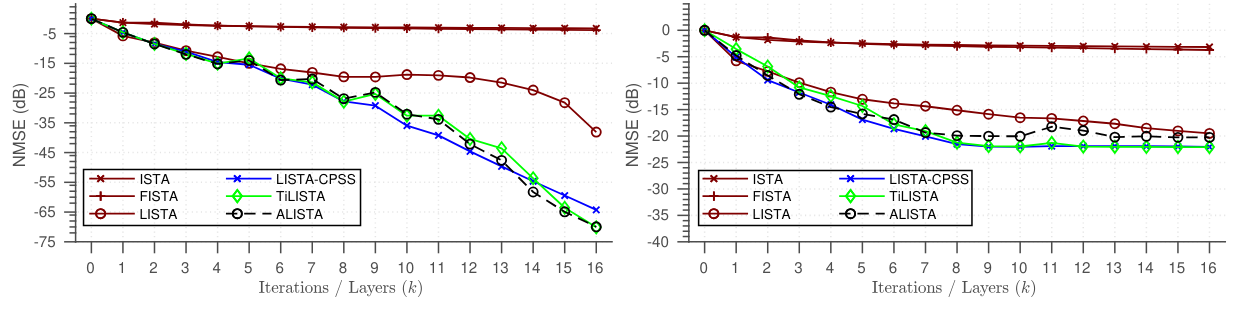
\includegraphics[width=\textwidth]{./Figures/lista.png}
  \caption{L2O optimizers (LISTA, LISTA-CPSS, TiLISTA and ALISTA) converge much faster than the two popular iterative solvers (ISTA, FISTA). Left: noiseless case. Right: noisy case (SNR = 20). Source: \cite{liu2019alista}}
  \label{fig: lista}
\end{figure}

Model-Based DL is also deeply linked with the idea of \textit{L20} \cite{chen2022learning}, an emerging approach that leverages machine learning to develop optimization methods, aiming at reducing the laborious iterations of hand engineering. It automates the design of an optimization method based on its performance on a set of training problems. When it comes to problems where the target solutions are difficult to obtain, such as nonconvex optimization and inverse-problem applications, the solution of a well-trained L2O method can have better qualities than those of classic methods. However, it's imperative to note that the L2O or Model-Based DL is suitable for repeatedly solving a particular optimization problem over a specific distribution of data, while it typically fails on out-of-distribution problems. Thus its practicality depends on the type of target optimization, the chosen architecture of the method to learn, and the training procedure. To conclude the following Figure \ref{fig: overview} nicely depicts each of the three methods, i) Model-Based, ii) Data-Driven Deep Learning and finally iii) Model-Based Deep Learning. 

\begin{figure}[htbp]
  \centering
  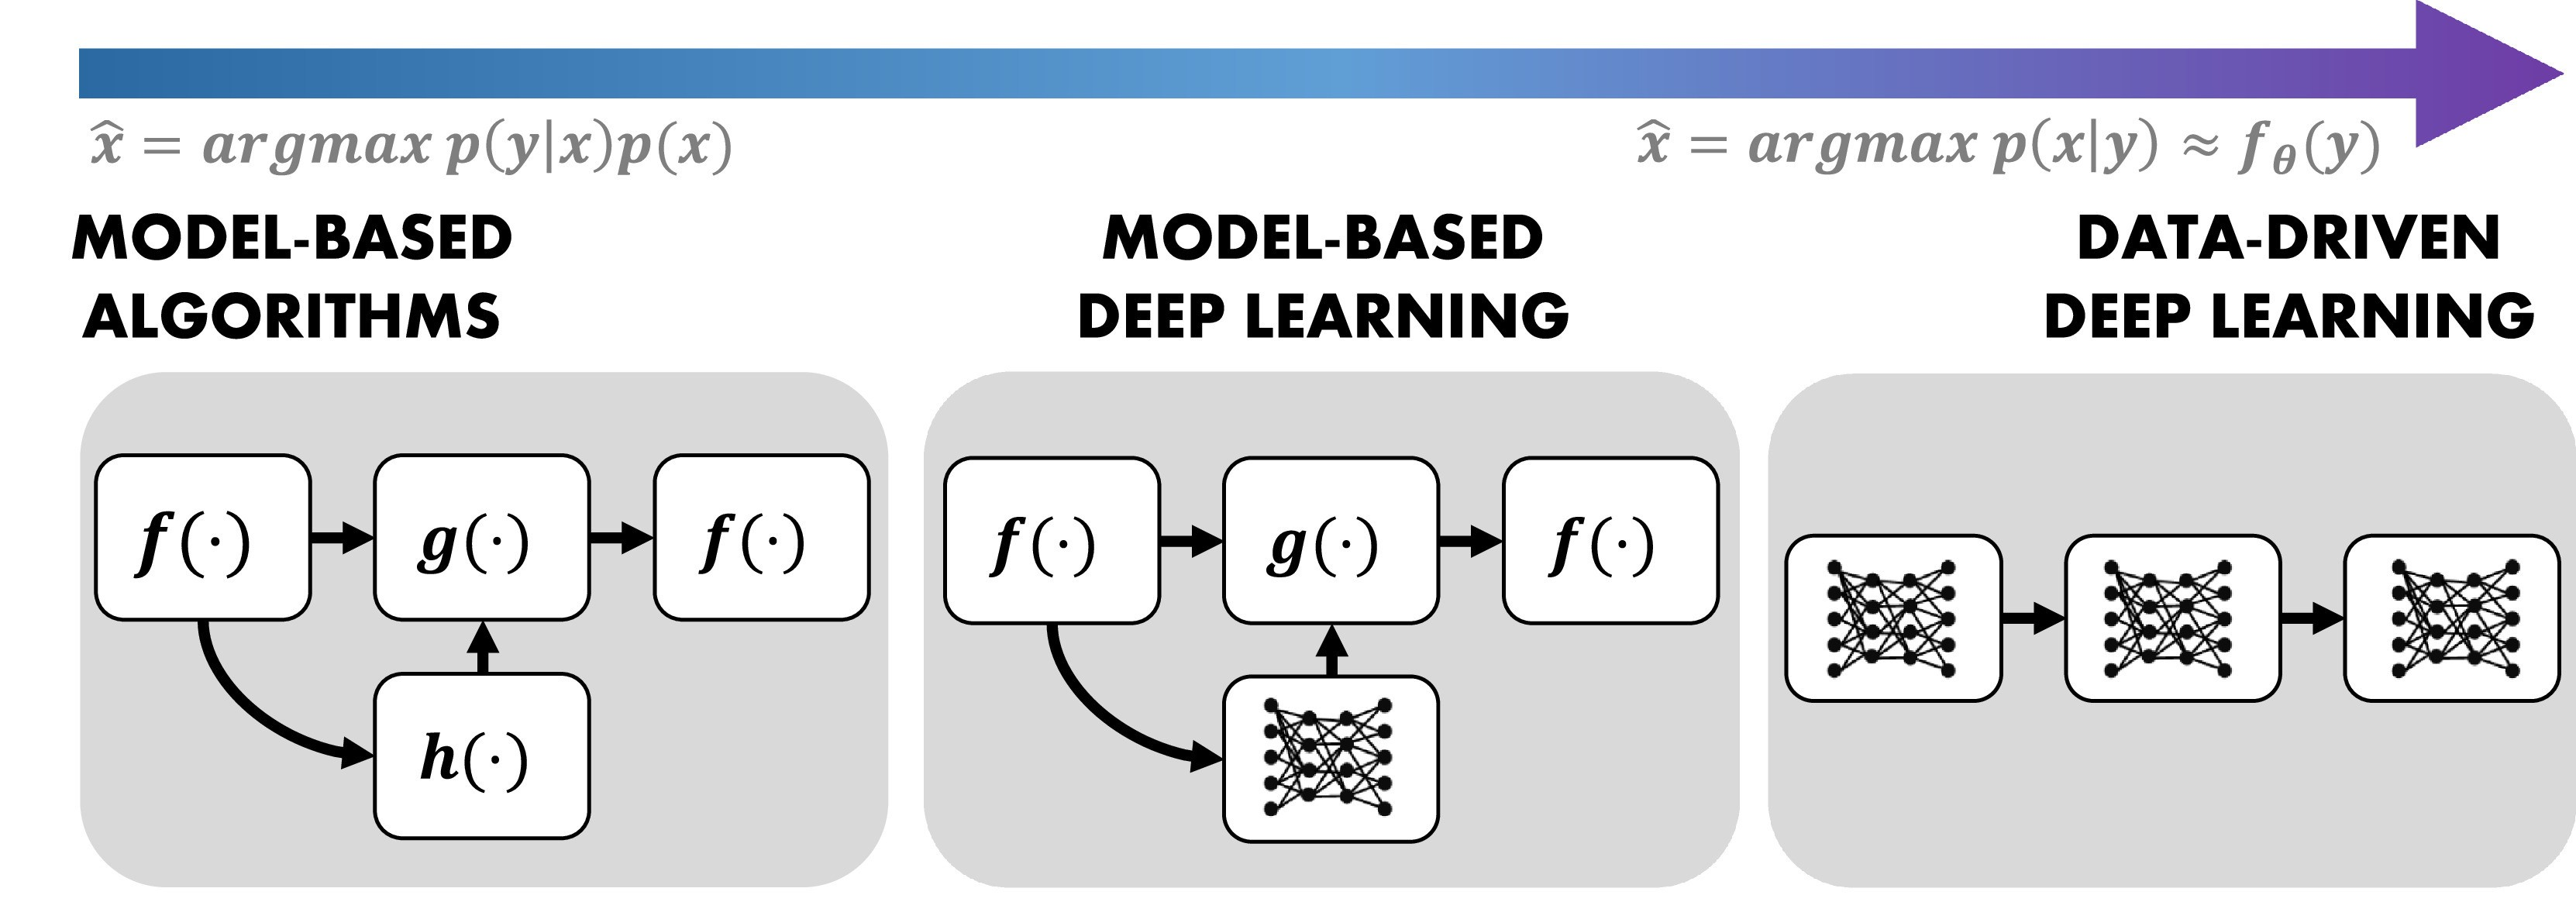
\includegraphics[width=\textwidth]{Figures/overview.jpg}
  \caption{Schematic overview of model-based and deep learning. Source: \cite{LUIJTEN2023677}}
  \label{fig: overview}
\end{figure}


\section{Matrix Completion}

\subsection{Problem and Motivation}

During the past few years, matrix completion (MC) has received increasing interest worldwide for its unique property and numerous applications in traffic sensing \cite{traffic_sensing}, integrated radar and communications \cite{radar_communications}, image inpainting (more on it later) \cite{image_inpainting}, recommendation systems with the most common being the \textit{Netflix Prize} problem \cite{jackson2017netflix}, and so on. Subsequent to compressed sensing (CS), MC is another significant technology utilizing sparse property to process data. Sparsity, in CS, means that the signal of interest contains lots of zero elements in a specific domain. However, in MC, it indicates that the singular value vector of the original matrix is sparse. In other words, the matrix is \textit{low-rank}.

MC is able to restore the original signal $X$ from a fragmentary signal $X_{\Omega}$ (or called the undersampled/incomplete signal), where $\Omega$ is a subset containing $2D$ coordinates of sampled entries. The undersampled signal $X_{\Omega}$ can be expressed as:
\begin{equation}
    X_{\Omega} = H_{\Omega} \odot X + N \label{eq: 8}
\end{equation}

\[
H(i, j) = 
\begin{cases}
1 & \text{if } (i, j) \in \Omega \\
0 & \text{otherwise}
\end{cases}
\]
where all variables belong to $\mathbb{R}^{n \times m}$, $\odot$ is the element wise multiplication (Hadamard) operator, $H_{\Omega}$ and $N$ are the sampling matrix and noise matrix, respectively. Note that $H_{\Omega}$ is a binary matrix, which are drawn from a random uniform distribution to ensure at least one $1$-element in each row and column. Furthermore, it is assumed that the original signal $X$ has the low-rank or approximately low-rank property.

Low-rank property of signals is ubiquitous in real-world applications. For instance, data collection of wireless sensor networks (WSNs) \cite{wireless_sensor}.Spatio-temporal signals are time series collected over a certain spatial range \cite{spatial}. In many cases, the collected spatio-temporal data is incomplete because of the limited power supply or malfunctions \cite{missing_node}. Hence, recovery of spatio-temporal signals from incomplete data is a critical issue in WSNs.The main information conveyed by the measurement matrix is dominated by some largest singular values, whereas the remaining smallest singular values can be taken as zero without losing major information. Thus, the measurement matrix has an approximately low-rank structure.

It is proposed to utilize rank minimization problem to restore the original signal $X$. The MC problem under the noise-free environment is formulated as:
\begin{equation}
    \min_{M} \text{rank}(M), \quad \text{s.t.} \quad M_{\Omega} = X_{\Omega} \label{eq: 9}
\end{equation}

where $M \in \mathbb{R}^{m \times n}$, $X_{\Omega} = H_{\Omega} \odot X$, and $M_{\Omega}$ denotes the projection on $\Omega$. When the sampled signal is corrupted by noise, there is a need to constrain the noise level within an appropriate range. As a result, the MC problem can be expressed as:
\begin{equation}
    \min_{M} \text{rank}(M), \quad \text{s.t.} \quad \|M_{\Omega} - X_{\Omega}\|_F \leq \delta \label{eq: 10}
\end{equation}

where $X_{\Omega}$ is defined by Equation \ref{eq: 8}, $\|\cdot\|_F$ denotes the Frobenius norm of a matrix, and $\delta > 0$ is a tolerance parameter that limits the fitting error.

Unfortunately, the rank minimization problem is NP-hard since all algorithms for exactly solving \ref{eq: 9} and \ref{eq: 10} are doubly exponential in dimension $\max(m, n)$ in both theory and practice. This is why all state-of-the-art algorithms attempt to solve the \textit{approximate} problem of rank minimization. This is done by replacing rank minimization problem with a \textit{nuclear norm} minimization (NNM) problem. \cite{fazel2002matrix} proved that the nuclear norm is the convex envelope of rank, which turns out to be a convex relaxation and in turn enables one to efficiently solve the issue of rank minimization in MC. This convex relaxation is akin to the relaxation of $\ell_0$ minimization to $\ell_1$ minimization in CS \cite{candes2008introduction}.

Subsequently, Cand\`es and Recht proposed to solve the rank minimization problem in \ref{eq: 9} by the nuclear norm minimization problem, given as:
\begin{equation}
    \min_{M} \|M\|_*, \quad \text{s.t.} \quad M_{\Omega} = X_{\Omega} \label{eq: 11}
\end{equation}

where $\|\cdot\|_*$ is the nuclear norm of a matrix defined as the sum of singular values$ \| M \|_* = \sum_{i=1}^{\min\{m,n\}} \sigma_i(M)$.


\subsection{MC Formulations}
Various MC methodologies have been developed from different perspectives, with pros and cons. To facilitate readers, we present a brief summary of several well-known MC algorithms in Table \ref{tab:mc_algorithms}.

\begin{table}[H]
\centering
\caption{Summary of Matrix Completion Algorithms}
\label{tab:mc_algorithms}
\begin{tabular}{@{}lll@{}}
\toprule
NNM & Normal Situation & Outlier Situation \\ \midrule
Nuclear norm relaxation & Matrix factorization & $\ell_{p}$ norm minimization \\
Semidefinite programming & Minimum Rank Approximation & Adaptive outlier pursuing\\
Robust PCA &  &  \\ \bottomrule
\end{tabular}
\end{table}

We will only discuss methods for i) NNM, ii) matrix factorization and iii) $\ell_p$-norm minimization in this paper. RPCA will be briefly mentioned but later discarded due to its limitations.

\subsubsection{Nuclear Norm Minimization}
Based on NNM, the singular value thresholding (SVT) \cite{SVT} approach proposed to use a proximal objective of nuclear norm minimization is given as:
\[
\min_{M} \tau \|M\|_* + \frac{1}{2} \|M\|_F^2, \quad \text{s.t.} \quad M_{\Omega} = X_{\Omega} 
\]
where $\tau \geq 0$. Note that the parameter $\tau$ provides a tradeoff between the convex-non smooth nuclear norm and convex, smooth Frobenius norm. Such minimization problems that can be broken down that can be decomposed in this way are often solved by setting up the lagrangian:
\begin{equation}
    L(M, Y) = \tau \|M\|_* + \frac{1}{2} \|M\|_F^2 + \langle Y, M_{\Omega} - X_{\Omega} \rangle. \label{eq: 12}
\end{equation}

where $Y \in \mathbb{R}^{n \times m}$ is the lagrange multiplier. 
To solve \ref{eq: 12}, Cai et al. \cite{cai2010singular} introduced a proximity operator associated with the nuclear norm. In particular, a soft-thresholding operator $D_{\tau}$ is introduced, which is defined as:
\begin{equation}
    D_{\tau}(Y) := U D_{\tau}(S) V^T, \quad D_{\tau}(S) = \text{diag}\{(\sigma_i - \tau)^+\}_{i=1}^r,
\end{equation}

where $r$ is the rank of $Y$, $Y = USV^T$ is the singular value decomposition (SVD) of $Y$ with $S = \text{diag}\{\sigma_i\}_{i=1}^r$, $U \in \mathbb{R}^{n \times r}$ and $V \in \mathbb{R}^{m \times r}$ being orthonormal matrices, and $(t)^+ = \max(0, t)$. Notably, each iteration in solving \ref{eq: 12} requires calculating the SVD of $Y$ and then obtaining $D_{\tau}(Y)$. This will be one of the main points we take into consideration later on when devising a model to unfold. 

\subsubsection{Robust PCA}
Lin et al. \cite{rpca} considered the MC problem as a special case of robust principal component analysis (PCA) problem and formulated it as:
\begin{equation}
    \min_{M} \|M\|_*, \quad \text{s.t.} \quad M + S = X_{\Omega}, \quad S_{\Omega} = 0 \label{eq: 13}
\end{equation}

where $S \in \mathbb{R}^{n \times m}$ is a sparse matrix. The inexact augmented Lagrange multipliers (IALM) \cite{rpca} solves the augmented Lagrange version of the above to obtain the result $M$. However, this approach does not consider the noisy environment due to $S_{\Omega} = 0$, thereby prohibiting its applications.

Based on the weighted nuclear norm \cite{wnnm}, the variant of robust PCA for MC was devised in \cite{wnnm}, which is formulated as:
\begin{equation}
    \min_{M} \|M\|_{w,*}, \quad \text{s.t.} \quad M + S = X_{\Omega}, \quad S_{\Omega} = 0 \label{eq: 14}
\end{equation}

It should be noticed that although the standard robust PCA for low-rank matrix recovery is able to process impulsive noise, the robust PCA for MC in \ref{eq: 13} and \ref{eq: 14} is not robust against impulsive noise. The standard robust PCA is formulated as:
\begin{equation}
    \min_{L,S} \|L\|_* + \lambda \|S\|_1, \quad \text{s.t.} \quad L + S = D \label{eq: 15}
\end{equation}

where $L \in \mathbb{R}^{n \times m}$ is the target matrix with low-rank property, $\lambda > 0$. Interestingly, $S$ in the constraint of \ref{eq: 15} can be taken as impulsive noise added to $L$. Accordingly, its sparse property can be characterized by the $\ell_1$-norm. Therefore, the standard robust PCA is robust against impulsive noise whereas its variant for tackling the MC problem does not retain this robustness. Actually, if the sampled entries in \ref{eq: 13} are corrupted by additive noise, the noise term cannot be suppressed due to $S_{\Omega} = 0$. This is why the robust PCA for MC has a bad performance in the case of noise, not to mention impulsive noise.

Although the MC approaches are capable of offering superior performance by tailoring the nuclear norm minimization criterion, they suffer from low computational efficiency and limited scalability in big-scale data. To circumvent this issue, the \textit{matrix factorization} (MF) \cite{matrix_factorization} was proposed to solve the MC problem without SVD. The basic idea behind the MF methodology is to utilize two low-rank matrices ($U \in \mathbb{R}^{n \times r}$ and $V \in \mathbb{R}^{m \times r}$) Denoting $M = UV$, yields the following optimization problem:
\[
\min_U \min_V \| (UV^T)_{\Omega} - X_{\Omega} \|_F^2
\].

We discuss how these types of structures are solved later on. 

\subsubsection{$\ell_p$-Norm Minimization}
Consider the case for impulsive noise which usually corrupts the received data in real-world applications. The $\ell_2$-norm cannot exactly characterize the behaviors of both impulsive and Gaussian noises. It is easy to understand this statement because the $\ell_2$-norm may seriously amplify the power of impulsive noise, which is much larger than the power of Gaussian noise. This thereby motivates one to exploit other metrics for the impulsive noise scenario. For a matrix $R$, $\ell_p$-norm is defined as:
\[
\|R\|_{p} = \left( \sum_{i,j} |R_{i,j}|^p \right)^{\frac{1}{p}}
\]
where $[R]_{i,j}$ is the element of $R$.

$\ell_p$-norm with $0 < p < 2$ is able to resist outlier and thereby has been widely adopted to handle the impulsive noise. This is because, roughly speaking, $|[R]_{i,j}|^p$ measures the level of our dislikes of $R_{i,j}$. If $|R_{i,j}|^p$ is very small, it does not affect the recovery performance. If $|R_{i,j}|^p$ becomes large, however, it is indicated that we have to handle strong dislikes for these large residuals. Dislikes correspond to the values we need to minimize. For instance, compared with $|R_{i,j}|$, $|R_{i,j}|^2$ magnifies residuals, especially the residuals associated with outliers. In other words, to minimize the total residual, $\ell_p$-norm ($0 < p < 2$) pays more attention to minimize large residuals, i.e., outliers. Consequently, $\ell_p$-norm ($p = 1$) has a better performance than $\ell_2$-norm.

The $\ell_p$-regression ($\ell_p$-reg) algorithm \cite{lp_reg} combines the MF technique and $\ell_p$-norm to solve the MC problem, which is formulated as:
\[
\min_{U,V} {\|(UV^T)_{\Omega} - X_{\Omega}\|}_{p}^{p}, \quad \text{s.t.} \quad 0 < p < 2
\]
Note that if $p = 2$, we reduce the problem to a least square solution. Details skipped but we employ the Iterative Reweighted Least Squares Algorithm (IRLS) \cite{irls} for $1 < p < 2$. 

\subsection{Algorithms}
Numerous algorithms can be employed to solve the MC problems. In this section, we will review only one main technique of optimization - Alternative Direction Method of Multiplier (ADMM), which comes under \textit{non-gradient} approaches. Although there exists several others as shown in the Table below, the ones we discuss are relevant mostly to the algorithms/models we propose or compare our performance to. Moreover, Block Coardinate Descent (BCD) is similar to ADMM, one being an unconstrained optimization problem while the other being a constrained optimization problem.

\begin{table}[htbp]
\centering
\caption{A Summary of Optimization Methods}
\label{tab:optimization}
\begin{tabular}{@{}lll@{}}
\toprule
\multicolumn{1}{c}{\textbf{Gradient}} & \multicolumn{1}{c}{\textbf{Non-gradient}} \\ \midrule
GD &  BCD\\
APG  &ADMM  \\
BI  &  \\ \bottomrule
\end{tabular}
\end{table}

\subsubsection{Alternative Direction Method of Multiplier}

For constrained large-scale optimization problems, Gabay and Mercier \cite{ADMM} firstly introduced ADMM to tackle it.  According to the principle of ADMM, the constrained problem to be optimized can be expressed as
\begin{equation}
    \min_{X,Z} F(X) + G(Z) \quad \text{s.t.} \quad AX + BZ = C
    \label{eq: 16}
\end{equation}

where $F(X)$ and $G(Z)$ are convex, $X \in \mathbb{R}^{m \times r}$, $Z \in \mathbb{R}^{n \times r}$, $A \in \mathbb{R}^{p \times m}$, $B \in \mathbb{R}^{p \times n}$, and $C \in \mathbb{R}^{p \times r}$. The ADMM firstly converts \ref{eq: 16} to not only the Lagrangian but \textit{augmented} Lagrangian. 
\[
L_{\delta}(X, Y, Z) = F(X) + G(Z) + Y^T (AX + BZ - C) + \frac{\delta}{2} \|AX + BZ - C\|_F^2
\]

where $\delta > 0$. Then, the BCD approach is employed to optimize $X$, $Y$, and $Z$ separately. Algorithm \ref{algo: 1} summarizes the ADMM approach.

Notice how compared to the lagrangian we set up in \ref{eq: 12}, we have an extra term 'augmented' to the objective function $\frac{\delta}{2} \|AX + BZ - C\|_F^2$ which acts like the usual regularization and enforcement of the constraints we see in typical linear or logistic regression. 

\begin{algorithm}
  \caption{ADMM}
  \begin{algorithmic}[1]
    \State \textbf{Input:} Maximum iteration $N$, $X_0, Z_0$ and $\delta$
    \For{$k = 0, 1, ..., N$}
      \State $X_{k+1} = \text{arg} \min_{X_k} L_{\delta}(X_k, Y_k, Z_k)$
      \State $Z_{k+1} = \text{arg} \min_{Z_k} L_{\delta}(X_{k+1}, Y_k, Z_k)$
      \State $Y_{k+1} = Y_k + \delta(AX_{k+1} + BZ_{k+1} - C)$
    \EndFor
    \State \textbf{Output:} $X_{k+1}, Z_{k+1}$
  \end{algorithmic}
  \label{algo: 1}
\end{algorithm}

Further, notice that ADMM carries out \textit{dual ascent} update for the lagrange multuplier $Y$. This is because, the augmented Lagrangian method seeks a saddle point of $X$ and $Z$ by alternating between minimizing with respect to the primal variable $X$ and $Z$ and taking one step of gradient ascent to increase $X$ using the dual variable $Y$ \cite{Wright-Ma-2022}. 

The rest of the process is similar to that of BCD i.e. finding the optimal estimates of the parameters in a distributed manner, which significantly enhances the computational efficiency. The main principle behind the BCD and consequently ADMM algorithm is to optimize one parameter set while keeping other parameter sets unchanged at one time.

\section{Model-Based Deep Learning and Matrix Completion}

Despite the usefulness of this approach, it has rarely been employed to solve matrix completion problems that are pertinent in signal processing, wireless sensor networks, recommendation systems, and other domains. From what we have seen, ADMM-Net \cite{admm-net} and DMFC-Net\cite{ma2022deep} are the only ones who have applied this method for such problems and both have shown impressive results. Recently, there has also been an interest in reconstructing images and other forms of data that have been corrupted with impulsive GMM noise, but all of these have proposed iterative solutions that are subject to the aforementioned problems. Deep unfolding, however, has the potential to set a new benchmark for results in matrix completion problems, as indicated by its application in other domains. In the following section, we propose our idea and how it has the potential to perform better in terms of inference and accuracy when compared to the state of the art algorithms.



% \begin{thebibliography}{9}
% \bibitem{candes2010power}
% Candès, E.J., and Tao, T. (2010). The Power of Convex Relaxation: Near-Optimal Matrix Completion. \textit{IEEE Trans. Inf. Theory}, 56(5), 2053–2080.
% \bibitem{cai2010singular}
% Cai, J.F., Candès, E.J., and Shen, Z. (2010). A Singular Value Thresholding Algorithm for Matrix Completion. \textit{SIAM J. Optim.}, 20(4), 1956–1982.
% \bibitem{recht2010guaranteed}
% Recht, B., Fazel, M., and Parrilo, P.A. (2010). Guaranteed Minimum-Rank Solutions of Linear Matrix Equations via Nuclear Norm Minimization. \textit{SIAM Rev.}, 52(3), 471–501.
% \bibitem{jiang2019nonconvex}
% Jiang, H., Lu, Z., Lin, Z., and Zhang, C. (2019). Nonconvex Matrix Factorization from Rank-One Measurements. \textit{SIAM J. Optim.}, 29(1), 693–721.
% \bibitem{candes2011robust}
% Candès, E.J., Li, X., Ma, Y., and Wright, J. (2011). Robust Principal Component Analysis? \textit{J. ACM}, 58(3), Article 11, 37 pages.
% \bibitem{lin2010augmented}
% Lin, Z., Chen, M., and Ma, Y. (2010). The Augmented Lagrange Multiplier Method for Exact Recovery of Corrupted Low-Rank Matrices. \textit{arXiv preprint arXiv:1009.5055}.
% \bibitem{chen2011robust}
% Chen, Y., and Wiesel, A. (2011). Robust subspace recovery by weighted nuclear norm minimization. \textit{IEEE Trans. Inf. Theory}, 57(6), 3515–3529.
% \end{thebibliography}
 % What to Write 

% Chapter 3

\chapter{Methodology and Tools} % Write in your own chapter title
\label{Chapter3}
\lhead{} % Write in your own chapter title to set the page header

\section{Pipeline 1 - ConvMC-Net}
\subsection{General Methodology}
% We reverted to convolution maps as that has been shown to perform amazingly well in deep unfolded approaches (maybe cite some resouces like ISTA being unfolded etc) So now borrow content from shoaib bhai paper of ConvMC and mention the classic augmented lagrangian approach + CNNs to give rise to ConvMC net. Mention how it was trained (from synthetic generation - explain breifly i.e. the vanilla problem with simple white noise so far). Can even show the architecture diagram as well here. 
Now that we have discussed in quite detail the various algorithms and optimization techniques for matrix completion problem and the essence of model-based deep learning, we propose \textit{ConvMC-Net} our first model combining the systematic connections built in the already fine-tuned optimization algorithm namely ADMM (discussed in previous chapter) and unprecedented performance gains we aim to gain from the inclusion of deep learning methods. 

As the name suggests, ConvMC-Net uses learnable convolution kernels, which are learned from data, in its unfolding process. We trained our model on two tasks, i) Synthetic Dataset and ii) Image Inpainting. We utilized the unfolding of a \textit{vanilla} formulation with no noise component in our objective function. This was done mainly to test how much one can trust the 'learning' paradigm even when it will be faced with 'seemingly' out of distribution problems i.e. matrix recovery in the presence of noisy entries. More details later in section 3.1.3.

The synthetic dataset ground labels were constructed from a product of two normal distributed matrices and then a mask of same shape as the product with entries of 1/0 randomly chosen was multiplied to give the low-rank matrix. We varied the level of white noise (variance) and the sampling rate to get various datasets. Further, seeing that matrix completion problems are prevalent in wireless sensor networks, we also trained the model on a on a real-world sensing dataset. It consists of temperature data collected every 30 seconds by 54 sensors distributed in Intel Berkeley Research Lab \cite{intelberkeley2004}. Further, for image inpainting we resorted to using the CSDS 300 Color dataset \cite{MartinFTM01} consisting of 200 train images and 100 test image.. The training process used the original matrices as the ground truth and low-rank as the input. Finally, as discussed in detail later in section 3.1.3, we transitioned from a simple white noise to GMM noise, a problem that is recently being dealt when it comes to robust matrix completion for e.g \cite{lo-bcd}. This is not the end for our dataset creation methods as during our experimentation, we found several algorithms performing better/worse if the matrix dimensions were to increase/decrease. Hence we resorted to the above datasets in two formats i) $150 \times 300$ and ii) $400 \times 500$. 

For comparison purposes we resorted to first dealing with a similar deep unfolding approach (mentioned before) of ADMM-Net. Our experiments on a real world dataset of a sensor network show that the proposed ConvMC-Net is significantly faster than ADMM-Net in both training and at inference while giving better accuracy and showing improved robustness. Moreover, the number of layers of ConvMC-Net can be increased very easily for improved convergence, if needed, and it is also easily applicable on high dimensional matrices. Therefore, we later switched to comparing with other several prominent algorithms. 

\subsection{Data Selection}

For a problem as matrix completion or any other low rank approximation or matrix factorization or mostly any problem that can be formulated as a matrix recovery problem through regression or other such frameworks, synthetic datasets provide an amazing flexibility. Not only it is simple, straightforward but we can theoretically generate as many samples we want. For this reason, as well as other prominent methods, they always test their performance on synthetic datasets before going for challenging their models in real-life scenarios such as image inpainting or hyperspectral imaging. The synthetic dataset generation for GMM noise is explained below. Note the case for simple white gaussian noise was similar except the pdf of the noise changed from a GMM pdf to simple normal distribution. 

The noise-free and complete matrix $X \in \mathbb{R}^{400 \times 500}$ with $r = 10$ is generated by the product of $X_1 \in \mathbb{R}^{400 \times 10}$ and $X_2 \in \mathbb{R}^{10 \times 500}$ whose entries obey the standard Gaussian distribution. Then, the incomplete matrix without noise $X_{\text{incomplete}}$ consists of randomly selected 50\% entries from $X$. In other words, 50\% entries of $X_{\text{incomplete}}$ are equal to 1, and the rest are 0. Moreover, $X_{\text{incomplete}}$ is added with independent impulsive noise which is modeled by Gaussian mixture model (GMM). The probability density function (PDF) of GMM is given by
\[
p_v(v) = \frac{c_1 }{\sqrt{2\pi\sigma_1^2}} \exp\left(-\frac{v^2}{2\sigma_1^2}\right) + \frac{c_2}{ \sqrt{2\pi\sigma_2^2}}\exp\left(-\frac{v^2}{2\sigma_2^2}\right)
\]
where $c_1 + c_2 = 1$ with $0 < c_i < 1$, and $\sigma_1^2$ and $\sigma_2^2$ are variances. To simulate the impulsive noise, it requires $\sigma_2^2 \gg \sigma_1^2$ and $c_2 < c_1$. It means that sparse and high power noise samples with $\sigma_2^2$ and $c_2$ are mixed in Gaussian background noise with small variance $\sigma_1^2$. In our simulations, we set $\sigma_2^2 = 100\sigma_1^2$ and $c_2 = 0.1$. The signal-to-noise ratio (SNR) is defined as
\[
\text{SNR} = \frac{\|X_{\text{incomplete}}\|_F^2}{\sigma_v^2}
\]
where $\sigma_v^2 = \sum_{i=1}^{2} c_i \sigma_i^2$ is the total noise variance.

The recovery performance is measured by mean squared error (MSE), defined as
\[
\text{MSE} = \frac{\|M - X\|_F^2}{mn}
\]
where $M$ is the recovered matrix.

We followed a similar process for the image inpainting dataset CSDS 300 which consisted of 200 train images and 100 test images. Each image was RGB format and 481 x 321 hence was appropriately gray-scaled, resized before passing it to the data generation above. 

As for the preperation of the real-world sensing dataset, its laid down in Chapter 4. 

\subsection{Deep Learning Architecture and Final Design}

% Explain in detail the the architecture starting from the problem formulation toaugmented lagrangian to ALM algorithm to CNN utilization (basically shoaib paper stuff). But in this section in detail explain the slump we faced here when comparing results on image inpainting/synthetic datasets with the GOAT L0-BCD (vanilla problem vs GMM noise problem) which eventually led us to M-estimation. But also mention we later tried it on GMM corrupted data as well (synthetic + image inpainting both but very sus results i.e. same trajectories of loss)
In this section, we go through the technical details of our model ConvMC-Net and its first competitor ADMM-Net. We start of with the formulation of ConvMC-Net derived from the vanilla problem structure solved through \textit{augmented Lagrange multiplier} method. 

MC aims at restoring the original matrix $D_{M \times N}$ from its undersampled/incomplete version $D_{\Omega}$, expressed as
\[ D_{\Omega} = U \odot D, \]
where $\Omega$ is a subset containing 2D coordinates of sampled entries, $\odot$ represents the Hadamard product, and $U$ represents the sampling matrix. Furthermore, it is assumed that $D$ is low-rank. NNM setup is the following:
\[
\min_L \|L\|_*, \text{ such that } D_{\Omega} = L_{\Omega},
\]
where $\|.\|_*$ represents the nuclear norm of a matrix defined as the sum of the singular values of $L$, and $L_{\Omega}$ denotes the projection on $\Omega$. We formulate above in an augmented Lagrangian form as
\begin{equation}
    L(L, Y) = \|L\|_* + \text{Tr}(Y^T \cdot (D_{\Omega} - L_{\Omega})) + \frac{\mu}{2} \|D_{\Omega} - L_{\Omega}\|_F^2,
\label{eq: 22}
\end{equation}

where $\|.\|_F$ denotes the Frobenius norm, $\text{Tr}()$ denotes the trace of a matrix, $Y$ is the Lagrange multiplier of size $M \times N$, and $\mu$ is a regularization parameter that controls the penalty for violation of linear constraints. The augmented Lagrangian method seeks a saddle point of $L$ by alternating between minimizing with respect to the primal variable $L$ and taking one step of gradient ascent to increase $L$ using dual variable $Y$ as
\begin{equation}
    L^{k+1} \in \min_L \frac{1}{\mu} \|L\|_* + \frac{1}{2}  \|D_{\Omega} - L_{\Omega} + \frac{Y}{\mu}\|_F^2,
    \label{eq: 17}
\end{equation}

\[ 
Y^{k+1} = Y^k + \mu \nabla_Y L(L^{k+1}, Y^k),
\]
where $\nabla_Y L(L^{k+1}, Y^k)$ denotes the gradient of \ref{eq: 22} with respect to $Y$. We then solve \ref{eq: 17} using ISTA, the iterative step of which is given as
\begin{equation}
    L^{k+1} = \text{prox} \left( L^k - \frac{1}{\mu} \nabla_L L^k \right),
    \label{eq: 18}
\end{equation}

where $\text{prox} (.)$ denotes the proximal operator and $\nabla(L)$ denotes the gradient of the quadratic part with respect to $L$. The proximal operator for computing the low-rank component is the singular value thresholding operation, $\Psi_{\alpha}(X) = U \text{diag}(\text{Relu}(\sigma_i - \alpha))V^H$, where $X$ has an SVD given by $X = U\Sigma V^T$, $\text{diag}(y_i)$ represents a diagonal matrix with its $i^{th}$ diagonal entry equal to $y_i$, and $\sigma_i$ represents the $i^{th}$ singular value of $X$. The resulting procedure is stated in Algorithm 5. 

\begin{algorithm}
\caption{Matrix Completion by ALM}
\begin{algorithmic}[1]
\State \textbf{Input:} Initialize: $L^0 = Y^0 = 0$, $\mu > 0$
\State \textbf{Output:} $L$
\While {not converged}
    \State $L^{k+1} = \Psi_{\mu^{-1}} \left\{ L_{\Omega^C} + D_{\Omega} + \mu^{-1}Y_{\Omega} \right\}$, where $\Omega^C$ denotes the complement of set $\Omega$
    \State $Y^{k+1} = Y^k + \mu(D_{\Omega} - L^{k+1}_{\Omega})$
\EndWhile
\State \textbf{Return} $L$
\end{algorithmic}
\label{algo: 2}
\end{algorithm}

Although there are different ways \cite{way1, way2, way3} to unfold an iterative algorithm into a DNN, we follow the method of \cite{way1} in unfolding Algorithm \ref{algo: 2}. Hence, we introduce a measurement matrix $H$ into \eqref{eq: 17} as follows:
\begin{equation}
\min_L \frac{1}{\mu} \|L\|_* + \frac{1}{2} \|D_{\Omega} - (HL)_{\Omega} + \frac{Y_{\Omega}}{\mu}\|_F^2 \label{eq: 19}
\end{equation}
We further replace $(HL)_{\Omega}$ with $GL_{\Omega}$ on the basis that there exists a matrix $G$, corresponding to $H$, such that $\|(HL)_{\Omega} - GL_{\Omega}\|_F < \epsilon$. Using \ref{eq: 18}, the iterative step for $L$, after some algebraic manipulation, turns out to be:
\begin{equation}
\begin{aligned}
L^{k+1} = &\Psi_{\frac{1}{\mu^k}} \{L^{k} + G^T D_{\Omega} - G^T G L^{k}_{\Omega} + \frac{G^T}{\mu^{k}} Y^{k}_{\Omega} \}
\end{aligned}
\label{eq: 20}
\end{equation}
We unroll \ref{eq: 20} into the multi-layer neural network of ConvMC-Net by replacing the functions of the matrix $G$ with learnable parameters. Consequently, we replace $G^T$ and $G^T G$, multiplied with $D_{\Omega}$ and $L^{k}_{\Omega}$, respectively with convolution kernels.

In case of the Lagrange multiplier $Y$, we consider for a fixed $G$, two matrices $W$ and $B$ such that $G^T Y_{\Omega} = W \circ Y_{\Omega} + B$.

Finally, we write the deep unfolded version of \ref{eq: 20} as:
\begin{equation}
L^{k+1} = \Psi_{\frac{1}{\mu^{k}}} \{L^{k} + (C^{k}_{1} * D) + (C^{k}_{2} * L^{k}_{\Omega}) + (W_k \circ Y^{k}_{\Omega} + B^k)\}
\label{eq: 21}
\end{equation}
where $*$ denotes the convolution operation, $C^{k}_{1}$, $C^{k}_{2}$ are the convolution kernels learned in the $k$th layer of ConvMC-Net together with the matrices $W^k$ and $B^k$ and the regularization parameter $1/(\mu^k)$. Experimentation details such as epochs, etc are mentioned in chapter 4. We move on with the formulation of ADMM-Net. 

ADMM-Net is derived from unfolding the iterative steps for solving the following minimization problem:
\begin{equation}
\begin{aligned}
\min_{L,Z} & \rho \|Z\|_* + \frac{1}{2} \|D_{\Omega} - L_{\Omega}\|_F^2 + \frac{\lambda_1}{2} \|L^T\|_F^2 + \frac{\lambda_2}{2} \|SL\|_F^2, \\
& \text{such that } L = Z, \label{eq:admm-net-problem}
\end{aligned}
\end{equation}
where $\lambda_1$, $\lambda_2$, and $\rho$ denote the regularization parameters, $Z$ is a slack variable, $T$ represents a differential operator \cite{mao2018spatio} such that $LT = [l_2 - l_1, l_3 - l_2, ..., l_N - l_{N-1}]$, and $S$ represents the spatial relation among measurements of different sensors \cite{mao2018spatio} such that $SL$ gives the spatial difference of $L$. Minimizing $\|LT\|_F^2$ enforces temporal consistency of the sensor readings whereas minimizing $\|SL\|_F^2$ enforces spatial correlation between sensor readings. The deep unfolded steps of ADMM-Net are then written as
\begin{align}
\text{vec}(L^{k+1}) &= (\tilde{U} + \lambda^k_1\tilde{T} + \lambda^k_2\tilde{S} + \zeta^k\tilde{I})^{-1} \text{vec}(\zeta^k(Z^k - P^k)) + D_{\Omega}, \label{eq:admm-net-step1} \\
Z^{k+1} &= \Psi_{\tau^k} \left( L^{k+1} + P^k \right), \label{eq:admm-net-step2} \\
P^{k+1} &= P^k + \eta^k (L^{k+1} - Z^{k+1}), \label{eq:admm-net-step3}
\end{align}
where $\zeta$ is a penalty parameter introduced when making the augmented Lagrangian from \ref{eq:admm-net-problem}, $\tilde{I}$ is the $MN$ dimensional identity matrix, $P = M/\zeta$ where $M$ is the Lagrange multiplier, and $\tilde{U} = \text{diag}(\text{vec}(U))$. Furthermore, $\tilde{S} = I_N \otimes ((S_k)^T S_k)$ and $\tilde{T} = (T^T T) \otimes {I_M}$, where $\otimes$ represents the Kronecker product. The parameters $\{S^k, \lambda^k_1, \lambda^k_2, \zeta^k, \tau^k, \eta^k\}_{k=1}^K$ are learned by the network at every layer in ADMM-Net.

\section{Pipeline 2 - Huber Approach}
% Exact same subsections as above pipelines 
\subsection{General Methodology}
As already discussed much in chapter 2 about the approach of matrix factorization to solve matrix completion, we transitioned from the above ADMM to such an approach. This was done due to few reasons and had several benefits. The objective function above dealt with in both ADMM-Net and ConvMC-Net is a non-smooth convex optimization problem because of the presence of the nuclear norm. Moreover, due to such non-smooth techniques, techniques like ALM/ADMM are required which are further equipped with 'proximal' step updates to deal with the non-smooth term. This as we have seen above, requires the use of SVT. And since our main aim from the start was to improve accuracy but also as importantly as inference, we resorted to convex-optimization problem formulations that do not require such SVD calculations especially at each iteration of the algorithm. Moreover, as far as we have seen very few if not none have attempted at unfolding such smooth convex-optimization problems. One might infer it might be that DNNs love non-smooth updates like that of proximal updates and optimal updates found in convex problems are not so beneficial for DNNs to bank on. Again this was a hypothesis at the start and only through experimentation could we validate this claim. 

The last reason why we tried unfolding matrix factorization approaches is because the classic ADMM approach as seen in ConvMC-Net did not even have a sprinkle of noise assumed in its objective formulation. This is because as shown above that such methods are not equipped to deal with complex noise distributions especially GMM which is at the center of research right now. However, note that variants of such Principal Component Pursuit (PCP) methods do exist such as Accelerated Proximal Gradient \cite{apg} but that adds increased complexity. That can be a another research attempt for another time however, matrix factorization are flexible enough to deal with such complex noise distributions and do not require expensive computation like SVD. Therefore, this is why we tried to go ahead with the unfolding of such algorithms hoping for further improved inference and accuracy,

In general the methodology we adopt to unfold here unlike ConvMC-Net before with the inclusion of CNN's, we go ahead with one of the most prominent algorithm in fields of signal processing i.e. majorization-minimzation (MM) approach \cite{lange_mm_algorithm} based algorithm known as 'Huber' Regression. It employs one of the famous 'Huber Criterion' \cite{huber_criterion} as its smooth convex optimization problem effectively updating the matrix factors as sub-regression problems. More details regarding this algorithm, its unfolded version, its strong competitors \(\ell_0\)-BCD and \(\ell_p\)-reg will be discussed in much technical detail.

% start of by saying since we were comparing results with one of the top state of the art methods L0-BCD, we found it best to use of its tough competitiors through an unfolding approach. We came across M-Estimation techinque and Huber's Criterion a convex optimization problem with little to no computationally heavy operations like SVD. We utilized the MM algorithm in its iterative version (maybe link the Original huberreg - later proved to be wrong) by treating the matrix factorization as a simple regression problem. Training same as before but not on simple white noise data anymore but GMM corrupted data. 
\subsection{Data Selection}
We ignore this section for this pipeline as we follow the exact pipeline mentioned above in section 3.1.2. The details of the training process can be found in chapter 4. 
\subsection{Deep Learning Architecture}
% Explain in detail the algo (add it) and the architecutre (add pic if possible) of the original hubermc and its performance (again along the lines of fluctuation etc i.e. borrow content from section 4 of compilation). We then moved on the real hubereg found from our studies of Robust Signal Processing book etc mention the algorithm here followed by its unfolded architecture (with its cnns added) and its performance. Remember to include our tries of even learning X+. (failure performance - same performance throughout) 

We first discuss and motivate why one should adopt the MM method and Huber's criterion for a classical regression problem. Consider the following. 

Often the regression model also includes a constant term and, for this case, the model is
\[
y_i = \beta_0 + x_{[i]}^T\beta + v_i, \quad i = 1, \ldots ,N,
\]
where $\beta_0 \in \mathbb{F}$ is called the intercept. The model can be written in the form (2.7) by letting $x_{i} = (1, x_{i1}, \ldots , x_{ip})$, $i = 1, \ldots ,N$, be the vector of predictors for the $i$th response and $\beta = (\beta_0, \beta_1, \ldots , \beta_p)$ be the regression vector. When the vector notation of (2.8) is used, $X$ has size $N \times (p + 1)$, the first column being the $N$-vector of ones, denoted by $\mathbf{1}$. In this case, we let the column index of $X$ run from $0$ to $p$, so that $x_0 = 1$ and
\[
X = \begin{bmatrix}
x_0 & x_1 & \ldots & x_p
\end{bmatrix}.
\]
From now on, we assume a linear model with an intercept, unless mentioned otherwise.

Most criterion functions in regression seek to minimize the distance between $y$ and the fit $\hat{y}$, that is, the residual vector
\[
\hat{r} = y - \hat{y} = y - X\hat{\beta}
\]
should be as small as possible when a suitable metric is used. The most commonly used metric is the squared $\ell^2$-norm that leads to minimizing the residual sum-of-squares (RSS)
\[
\text{LRSS}(\beta) = \|y - X\beta\|_2^2 = \sum_{i=1}^N \left| y_i - x^{[i]}\beta \right|^2. \label{eq:rss}
\]

Minimization of $\text{LRSS}(\beta)$ is achieved by using the least squares estimate (LSE) $\hat{\beta}_{\text{LS}}$. The associated estimate for the scale parameter $\sigma$ of the error terms is the sample standard deviation,
\[
\hat{\sigma}_{\text{SD}}^2 = \frac{1}{N} \|\hat{r}\|_2^2 = \frac{1}{N} \sum_{i=1}^N \left| y_i - x^{[i]}\hat{\beta}_{\text{LS}} \right|^2, \label{eq:sd}
\]
or its unbiased version, $s^2 = \left[ \frac{N}{N - p - 1} \right] \hat{\sigma}_{\text{SD}}^2$. The LSE is the MLE for the Gaussian noise case, similar to how we developed it for an image denoising problem in Chapter 2.2 when discussing model-based approaches. However, it is also highly sensitive to outliers and is inefficient when the error terms are non-Gaussian. Hence robust loss criteria are necessary. Therefore, now we describe an elegant approach to estimate the unknown regression vector and scale using Huber’s criterion, which finds minimizers of a (jointly) convex criterion function $L_H(\beta, \sigma)$. We will skip most of the details regarding its formulation found in \cite {stat_book} and focus on key points. Note that most robust loss functions require an estimate of scale, and therefore joint estimation of the unknown regression vector $\beta$ and scale $\sigma$ is often desirable. The loss function we are going to discuss here is the \textit{Huber's Loss} function. 

Huber (1964) derived a family of univariate heavy-tailed distributions, which he called the least favorable distributions (LFDs). For the $\varepsilon$-contaminated Gaussian model, the LFD corresponds to a symmetric unimodal distribution that follows a Gaussian distribution in the middle and a double exponential distribution in the tails. The corresponding MLE is referred to as Huber’s M-estimator. Huber’s loss function is thus a hybrid of the $\ell_2$- and the $\ell_1$-loss functions defined previously, using the $\ell_2$-loss function for relatively small errors and $\ell_1$-loss function for relatively large errors. The pdf of the LFD has the form $f(x) = C \cdot (1/\sigma) \cdot \exp\{-\rho_{H,c}(x)\}$, where $\rho_{H,c}(x)$ is Huber’s loss \cite{huber_loss} function defined as
\[
\rho_{H,c}(x) = \begin{cases} \frac{1}{2}x^2, & \text{for } |x| \leq c \\ 2c|x| - c^2, & \text{for } |x| > c, \end{cases}
\]
where $c$ is a user-defined threshold that influences the degree of robustness. Huber’s function is convex and differentiable. Huber’s score function i.e. its derivative is of the form
\[
\psi_{H,c}(x) = \begin{cases} x, & \text{for } |x| \leq c \\ c \operatorname{sign}(x), & \text{for } |x| > c, \end{cases}
\]
Empirically the thresholds are chosen as $c_{0.95} = 1.345$ and $c_{0.85} = 0.7317$ for the real-valued case.

First, note that the ML approach for jointly solving the unknown parameters $\beta$ and $\sigma$ leads to minimizing the negative log-likelihood function:
\[
L_{\text{ML}}(\beta, \sigma) = N\ln \sigma + \sum_{i=1}^{N} \rho_{\text{H,c}} \left( \frac{y_i - x_i^T \beta}{\sigma} \right),
\]
The negative log-likelihood function, however, is not convex with respect to $(\beta, \sigma)$. This is easy to see by simply noting that $L_{\text{ML}}(\beta, \sigma)$ is not convex in $\sigma$ for a fixed $\beta$. Another problem is that even with a robust $\rho$ function, such as Huber’s loss function, the associated scale estimate will not be robust.

This is where the Huber criterion comes in as the following alternative criterion function
\[
\min_{\beta \in \mathbb{F}^{p+1}, \sigma > 0} L_{\text{HUB}}(\beta, \sigma) = N(\alpha \sigma) + \sum_{i=1}^{N} \rho \left( \frac{y_i - x[i] \beta}{\sigma} \right) \sigma,
\]
where $\rho$ is assumed to be a convex and differentiable loss function and $\alpha > 0$ is a fixed scaling factor that is used to obtain Fisher-consistency of $\hat{\sigma}$ when the errors are i.i.d. Gaussian ($v_i \sim \mathcal{N}(0, \sigma^2)$). We discuss later how $\alpha$ is computed. The minimizer $(\hat{\beta}, \hat{\sigma})$ of $L_{\text{HUB}}$ is referred to as hubreg estimates (of regression and scale) based on a loss function $\rho$.

An important feature of Huber’s criterion function is that it is jointly convex in $(\beta, \sigma)$ given that the loss function $\rho(\cdot)$ is convex. 

An important concept when dealing with hubreg estimates is that of the so-called pseudo-residual, which is associated with the score function $\psi(x) = \rho'(x)$ in the real-valued case and is defined as
\[
r_{\psi} \equiv r_{\psi}(\beta, \sigma) = \psi \left( \frac{y - X\beta}{\sigma} \right) \sigma,
\]
where the $\psi$ function acts coordinate wise on the vector $r/\sigma$, so $\psi(r/\sigma)_i = \psi(r_i/\sigma)$. Note that if $\rho(\cdot)$ is the conventional LS loss, then $\psi(x) = x$, and $r_{\psi}$ coincides with the conventional residual vector, so $r_{\psi} = y - X\beta = r$. The multiplier $\sigma$ in this definition is needed to map the residuals back to the original scale of the data.

Because the optimization problem is convex, the global minimizer $(\hat{\beta}, \hat{\sigma})$ is a stationary point of $L_{\text{HUB}}$. Thus, $(\hat{\beta}, \hat{\sigma})$ can be found by solving the M-estimating equations, obtained by setting the gradient of $L_{\text{HUB}}$ w.r.t. its arguments to zero. 

In order to use the MM algorithm there are some conditions that need to be met for e.g the convexity of $\rho(\cdot)$, however, we skip the proofs of these and straight jump to the algorithm. 

Concluding this, we have devised an MM algorithm that can be used to find the minimum $(\hat{\beta}, \hat{\sigma})$ of Huber’s criterion $L_{\text{HUB}}(\beta, \sigma)$, we employ the MM algorithm. The algorithm, named \texttt{hubreg}, is outlined in Algorithm \ref{algo: 3} below. This algorithm is specifically designed for the scenario where the loss function $\rho$ corresponds to Huber’s function.

\begin{algorithm}[H]
\caption{The \texttt{hubreg} algorithm for solving $L_{\text{HUB}}(\beta, \sigma)$ when $\rho = \rho_{H,c}$ using the MM algorithm.}
\begin{algorithmic}[1]
\Require $y \in \mathbb{F}^N$, $X \in \mathbb{F}^{N \times (p+1)}$, $c$, $\beta^{(0)}$, $\sigma^{(0)}$
\Ensure $(\hat{\beta}, \hat{\sigma})$, the minimizer of Huber’s criterion $L_{\text{HUB}}(\beta, \sigma)$ when $\rho = \rho_{H,c}$.
\State Initialize: $N_{\text{iter}} \in \mathbb{N}$, $\delta > 0$, $\alpha = \alpha(c)$ , $X^+ = (X^HX)^{-1}X^H$.
\For{$n = 0, 1, \dots, N_{\text{iter}}$}
    \State Update residual: $r^{(n)} = y - X\beta^{(n)}$
    \State Update pseudo-residual: $r_{\psi}^{(n)} = \psi_{H,c}\left(\frac{r^{(n)}}{\sigma^{(n)}}\right) \cdot \sigma^{(n)}$
    \State Update scale: $\sigma^{(n+1)} = \frac{1}{\sqrt{N(2\alpha)}} + r_{\psi}^{(n)} + \sigma^{(n)}$
    \State (Re)update the pseudo-residual: $r_{\psi}^{(n+1)} = \psi_{H,c}\left(\frac{r^{(n)}}{\sigma^{(n+1)}}\right) \cdot \sigma^{(n+1)}$
    \State Regress $X$ on $r_{\psi}^{(n+1)}$: $\delta^{(n)} = X + r_{\psi}^{(n+1)}$
    \State Update regression vector: $\beta^{(n+1)} = \beta^{(n)} + \delta^{(n)}$
    \If{$\frac{\delta^{(n)}}{\beta^{(n)}} < \delta$}
        \State \Return $(\hat{\beta}, \hat{\sigma}) \gets (\beta^{(n+1)}, \sigma^{(n+1)})$
    \EndIf
\EndFor
\end{algorithmic}
\label{algo: 3}
\end{algorithm}

Note that the scaling factor $\alpha$ in update scale is used to ensure that $\hat{\sigma}$ is Fisher-consistent for the unknown scale $\sigma$ when $\{e_i\}_{i=1}^N$ are i.i.d. $\sim N(0, 1)$. Skipping proof, this is achieved if
\begin{equation}
\alpha = E[c(e)] = \frac{c^2}{2} \left(1 - F_2^1(c^2)\right) + \frac{1}{2} F_2^3(c^2), \tag{8}
\end{equation}
where $F_2^k$ denotes the c.d.f. of the chi-squared distribution with $k$ degrees of freedom and $e \sim N(0, 1)$. Hence, when using the LS loss, $c(e) = \frac{1}{2} e^2$, and Fisher consistency is obtained if $\alpha = \frac{1}{2}E[e^2] = 1$.

Now we explain the above algorithm in the context of how it was used to address robust matrix completion. 

The observed matrix $X \in \mathbb{R}^{n_1 \times n_2}$ is modeled as
\[
X = M + S + N,
\]
where $M$ is a low-rank matrix of rank $r$, $S$ is an entry-wise sparse outlier matrix, and $N$ represents the background noise. Our goal is to recover the low-rank component $M$ from partially observed entries of $X$ corrupted by noise and outliers.

In our approach, the outlier-robust “norm” of $X$ is defined as
\[
\|X\|_{\sigma,c} = \sum_{i=1}^{n_1} \sum_{j=1}^{n_2} \rho\left(\frac{x_{ij}}{\sigma}\right),
\]
where $\sigma > 0$ is the scale parameter, $x_{ij}$ is the $(i, j)$th entry of $X$, and $\rho(\cdot)$ is a differentiable loss function. In this paper, we consider Huber’s loss function for which the associated tuning parameter $c$ trades off the efficiency and robustness. For example, $c = 1.345$ yield 95\% asymptotic relative efficiency for Huber’s loss Unlike the $\ell_1$-loss, Huber’s and Tukey’s losses are differentiable. Furthermore, Huber’s loss is convex.

To describe missing data, the row-column indices of the partially observed entries are collected in the set $\Omega \subset \{1, \ldots, n_1\} \times \{1, \ldots, n_2\}$. We use $X_{\Omega} \in \mathbb{R}^{n_1 \times n_2}$ to denote the projection of $X$ onto $\Omega$. As a result, we have $[X_{\Omega}]_{ij} = 0$ if $(i, j) \notin \Omega$ and $[X_{\Omega}]_{ij} = x_{ij}$ if $(i, j) \in \Omega$.

Now using similar matrix factorization technique as before, in the presence of outliers, our robust M-estimation based matrix completion is expressed as \cite{m-est}:
\[
\min_{U,V} \left\| (UV)_{\Omega} - X_{\Omega} \right\|_{\sigma,c}.
\]
Herein, the scale parameter $\sigma$ is unknown and is estimated jointly with $(U, V)$, whereas $c$ is set in advance and is considered constant. To solve the above equation, an alternating minimization strategy is applied. To be more specific, at the $(k + 1)$th iteration ($k = 0, 1, 2, \ldots$), $V$ and $U$ are alternately minimized:
\[
V^{k+1} = \arg \min_V \left\| (U^kV)_{\Omega} - X_{\Omega} \right\|_{\sigma,c}
\]
\[
U^{k+1} = \arg \min_U \left\| (UV^{k+1})_{\Omega} - X_{\Omega} \right\|_{\sigma,c}.
\]
Note that the above equations have the same structure. Thus, we only discuss how to solve the first equation, because the second equation is solved analogously. With the following definitions:
\begin{itemize}
    \item $u_i^{\top} \in \mathbb{R}^{1 \times r}$, and $v_j \in \mathbb{R}^{r}$, respectively denote the $i$th row of $U$ and $j$th column of $V$, where $i = 1, \ldots, n_1$ and $j = 1, \ldots, n_2$.
    \item $I_j = \{j_1, \ldots, j_{|I_j|}\} \subseteq \{1, \ldots, n_1\}$ represents the set containing the row indices for the $j$th column, $j = 1, \ldots, n_2$, of $\Omega$, where $\sum_{j=1}^{n_2} |I_j| = |\Omega|$, and, in general, $|I_j| > r$.
    \item $U_k^{I_j} \in \mathbb{R}^{|I_j| \times r}$ is the matrix containing the $|I_j|$ rows of $U_k$ that are indexed by $I_j$.
    \item $b_{I_j} = [x_{j1}, \ldots, x_{j|I_j|}]^{\top} \in \mathbb{R}^{|I_j|}$.
\end{itemize}
The optimization for $V$ can be rewritten as a series of robust linear regression problems that can be solved in parallel, i.e.,
\[
\min_{v_j} \left\{ f_{\sigma}(v_j) = \|U^k_{I_j} v_j - b_{I_j}\|_{\sigma,c} \right\}, \quad j = 1, \ldots, n_2.
\]
Since $\sigma$ is unknown and a preliminary estimate is difficult to obtain, we propose to solve the above equation using Huber’s joint M-estimation of regression and scale approach:
\[
\min_{v_j, \sigma > 0} L_{\text{hub}}(v_j, \sigma) = \sigma \sum_{i \in I_j} \rho_{\text{hub}} \left(\frac{x_{ij} - (u_i^T)^k v_j}{\sigma} \right) + |I_j| (\alpha \sigma),
\]
where $\alpha$ is a fixed scaling factor to obtain Fisher consistency of the scale estimate $\sigma$. Now, this is jointly convex in $(v_j, \sigma)$. Therefore, the global minimizer $(v_{bj}, \sigma_b)$ is a stationary point of Huber’s criterion, and a solution can be found by solving the M-estimating equations obtained by setting the gradient of $L_{\text{hub}}(v_j, \sigma)$, with respect to its arguments, to zero.

Finally, we get Algorithm \ref{algo: 4} for robust matrix completion using Huber's M-Estimation.

\begin{algorithm}[H]
    \caption{Robust Matrix Completion via Huber's M-Estimation}
    \textbf{Input:} $X_{\Omega}$, $\Omega$, and rank $r$ \\
    \textbf{Initialize:} Randomly initialize $U_0 \in \mathbb{R}^{n_1 \times r}$ \\
    Determine $\{I_j\}_{j=1}^{n_2}$ and $\{J_i\}_{i=1}^{n_1}$ according to $\Omega$
        \begin{algorithmic}
        \For{$k = 0, 1, \ldots$}
            \State // Fix $U_k$, optimize $V$
            \State $v^{k+1}_{j} = \arg \min_{v_j, \sigma} \left\{ \sigma \sum_{i \in I_j} \rho_{\text{hub}} \left(\frac{x_{ij} - (u_i^T)^k v_j}{\sigma} \right) + |I_j| (\alpha \sigma) \right\}$ for all $j = 1, 2, \ldots, n_2$
            \State // Fix $V_{k+1}$, optimize $U$
            \State $(u_i^T)^{k+1} = \arg \min_{u_i^T, \sigma} \left\{ \sigma \sum_{j \in J_i} \rho_{\text{hub}} \left( \frac{x_{ij} - (u_i^T)^k v_j^{k+1}}{\sigma} \right) + |J_i| (\alpha \sigma)  \right\}$ for all $i = 1, 2, \ldots, n_1$
            \State // Stop if a termination condition is satisfied
        \EndFor
        \end{algorithmic}
    \textbf{Output:} $M = U^{k+1}V^{k+1}$
    \label{algo: 4}
\end{algorithm}

Note how each non-zero subset of a specific column/row (depending on which matrix is being updated U, V) is being updated through a Huber regression problem formulation. Seeing that we have now discussed the algorithm for hubreg and how its iterative version plays out, we consider the proposed deep-unfolded version of hubreg in Figure \ref{fig: arch1}. 

\begin{figure}[htbp]
  \centering
  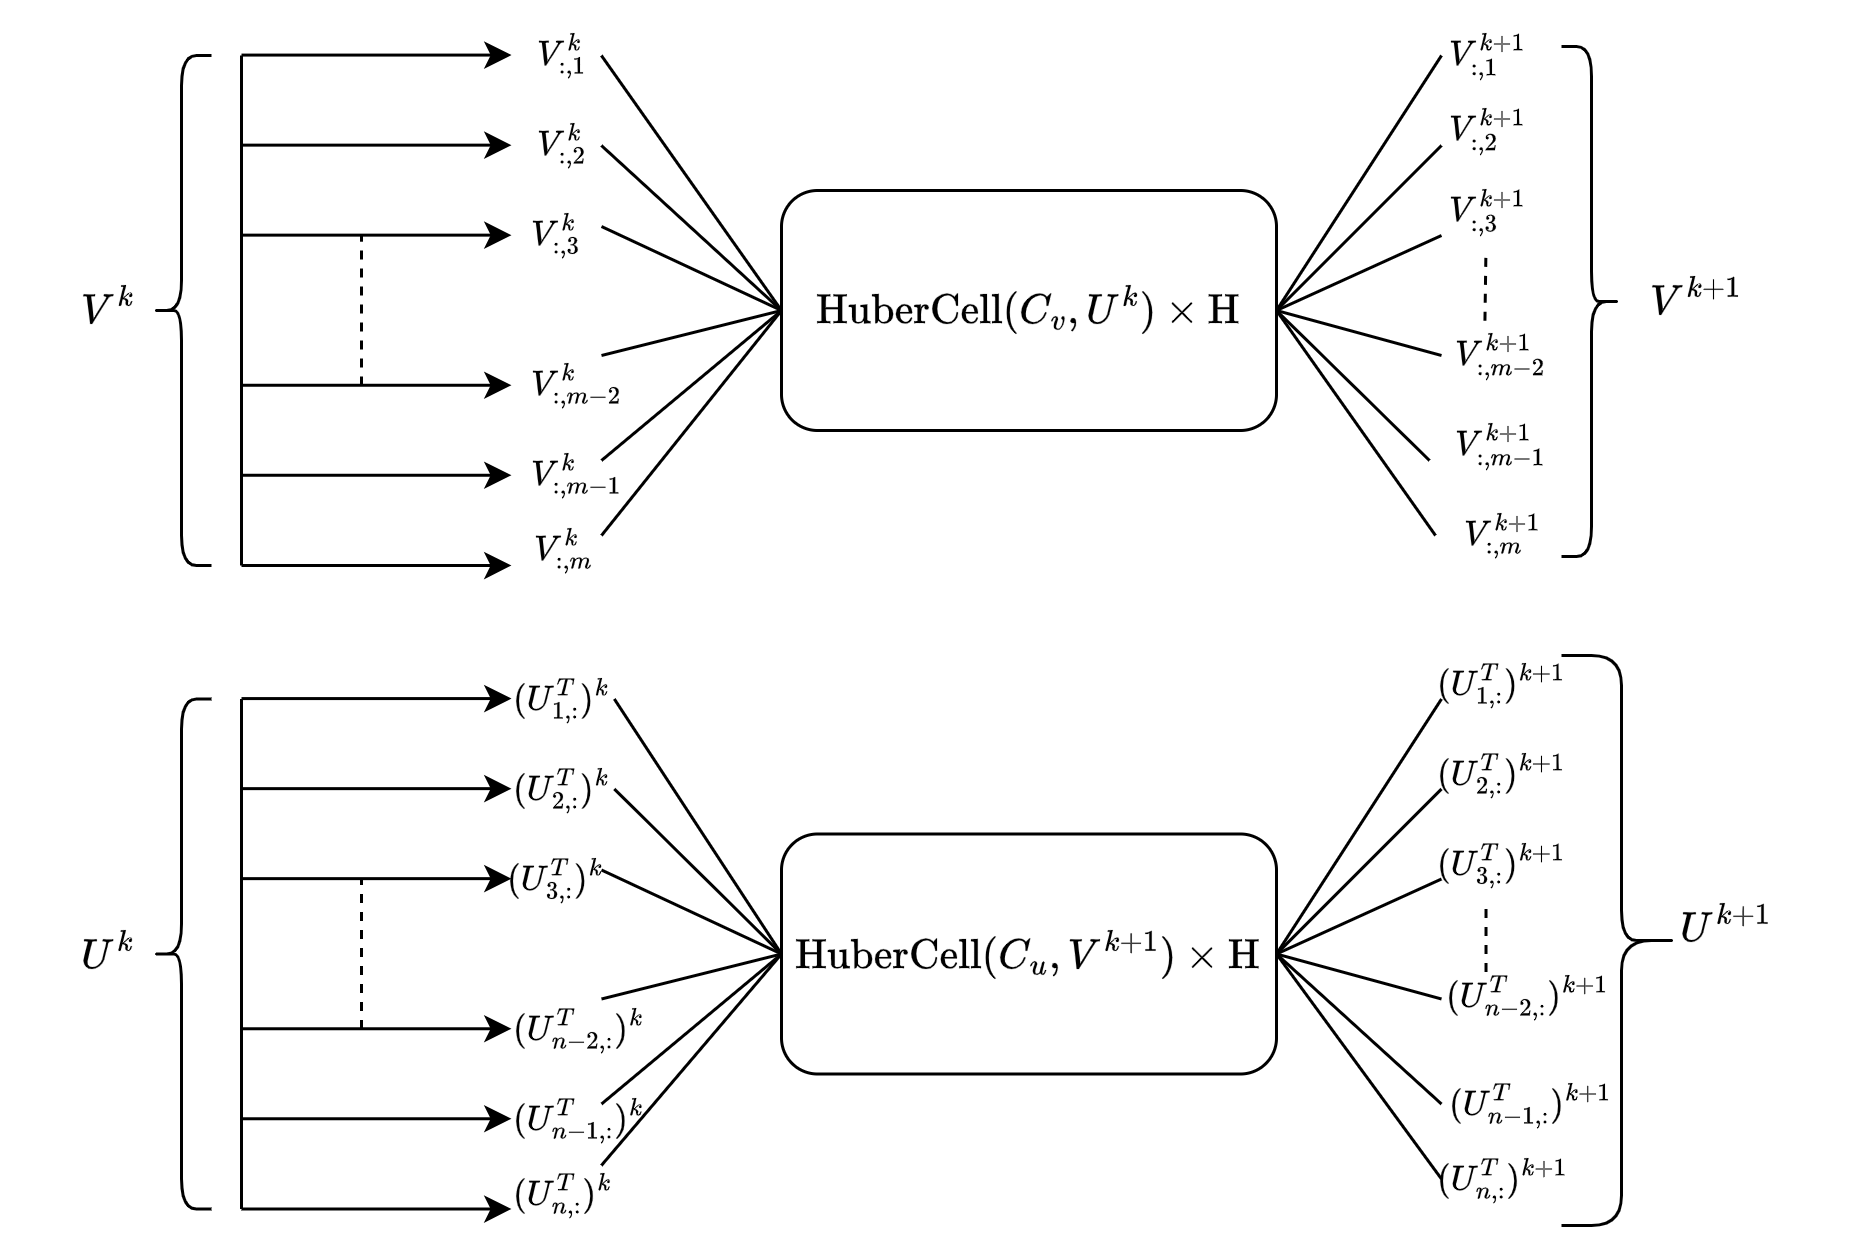
\includegraphics[width=\textwidth]{./Figures/huber-mc.png}
  \caption{ConvHuberMC-Net Architecture}
  \label{fig: arch1}
\end{figure}

We explain this architecture one by one. The neural network receives two inputs, $U$ and $V$ both initially randomly initialized from a standard normal. We then go ahead and sequentially update V followed by U. as shown in the above iterative version. Therefore by similarity, we consider the individuals columns of $V$, and rows of $U$. Each column of V and U go through a \textit{HuberCell} which is characterized by the exact Algorithm \ref{algo: 4} as discussed above. Note that each row/column update is accompanied by two arguments $C_i$ and current state of the other matrix. $C_i$ where $i \in {u, v}$ denotes the set of all learnable convolution maps (their hyperparameters such as stride etc discussed in section 4) for the matrix $U$ and $V$ respectively, all initialized to identity maps at the beginning for each update of row/column of $U$/$V$. Note that both matrix updates can be parallelized hence has much prospect in terms of computational ease. The convolution maps inclusion have been done in a very straightforward way by simply passing the convolution map to the corresponding $X^{+}$ for a specific update. This had two benefits. If we were to check the original paper of M-estimation being used to address RMC, the number of iterations $N_{iter}$ required for proper convergence was $500$. However, by making including these learnable parameters, we greatly reduce the number of iterations for a similar performance for some combinations as low as 2. This is precisely what $H$ denotes i.e. the $N_{iter}$ for a specific update. This is as simple as stacking HuberCells, one on top of another. In terms of computation ease, also note that the calculation of pseudoinverse only happens $H$ times compared to hundreds of times for the iterative version, again reducing the computational burden. 

After the HuberCell update, we get the updated column/row which are concatenated to form the updated U and V matrix. This update of U and V happens in same layer (\(k\)th layer as shown above). 

Now we go ahead and discuss briefly the state of the art methods \(\ell_0\)-BCD and \(\ell_p\)-reg.

\subsubsection{\(\ell_0\)-BCD Algorithm}

We will be going by the similar problem formulation as in \textbf{ALM} but this time we assume the sampled/incomplete matrix $D_{\Omega}$ has been exposed to impulsive Gaussian noise more specifically it can be decomposed as follows.

$$D_{\Omega} = \Tilde{D_{\Omega}} + G_{\Omega} + S_{\Omega}$$

where we consider the sampled and noisy matrix $D_{\Omega}$ can be decomposed into a noisy-free but sampled component $\Tilde{D_{\Omega}}$, Gaussian noise with small power/variance $G_{\Omega}$ and sparse impulsive Gaussian noises with high power, $S_{\Omega}$. We then formulate the \textit{robust} matrix completion (RMC) problem using matrix factorization and breaking the matrix of interest, $\Tilde{D_{\Omega}}$ into a product of two similar lower dimensional matrices, $U, V$.

\begin{equation}
\min_{U, V, S} \lVert D_{\Omega} - (UV)_{\Omega} - S_{\Omega} \rVert_F^{2} + \mu \lVert S_{\Omega} \rVert_0
\label{eq19}
\end{equation}
where $U \in \mathcal{R}^{M \times r}$ and $V \in \mathcal{R}^{r \times N}$
 and $r$ is the assumed rank of the original matrix $D$. 
Furthermore,  $S_0$ is utilized to separate outliers (sparse noise) from $D_{\Omega}$, and $\lVert D_{\Omega} - (UV)_{\Omega} - S_{\Omega} \rVert_F^{2}$ is able to resist the Gaussian noise, and $\mu > 0$ is the penalty parameter which controls the sparsity of $S$ and is automatically updated by a \textit{Laplacian} kernel-based method. \\ 

Using block coordinate descent (BCD) we are able to formulate this problem into further 3 sub-problems leading to the following iterative procedure: 

\begin{align}
U^{k+1} & = \arg \min_U \lVert D_{\Omega} - (UV^k)_{\Omega}  - S^{k}_{\Omega} \rVert_F^2 \\
V^{k+1} & = \arg \min_V \lVert D_{\Omega} - (U^{k+1}V)_{\Omega} - S^{k}_{\Omega} \rVert_F^2 \\
S^{k+1} & = \arg \min_S \lVert N^{k+1}_{\Omega} - S_{\Omega} \rVert + \mu^{k+1} \|S_{\Omega}\|_{0}
\end{align}

where $N^{k+1}_{\Omega} = D_{\Omega} - (U^{k+1}V^{k+1})_{\Omega}$. To solve (12) we use a hard-thresholding operator ${\tau}(\cdot)$ defined as follows: $$s^{k+1} = \tau_{\mu^{k+1}}(n^{k+1}) = \begin{cases}
(n^{k+1})_{i}, & \text{if} |(n^{k+1})_{i}| \geq \sqrt{\mu^{k+1}} \\
0, & \text{otherwise}
\end{cases}$$

We have used small letters $s$ and $n$ to denote their capital letter counterparts but with only non-zero entries. Mathematically, $s \in \mathcal{R}^{\|\Omega\|_{1}}$ and similarly $n \in \mathcal{R}^{\|\Omega\|_{1}}$. \\ Also note that after updating $U$ and $V$ we first update $\mu$ the adaptive penalty term before updating S. Without going into much detail how this is updated, the following algorithm summarizes the key steps in finding $\mu$ per iteration step. 

\begin{algorithm}
\caption{Outlier Detector Based on Laplacian Kernel}
\textbf{Input:} $n$ and $\epsilon$ \\
$\sigma^2 = 1.06 \times \min(\sigma_E, \frac{\text{IQR}}{1.34}) \times \text{dim}(n)^{-0.2}$ \\
$w = k_{\sigma}(n)$ \\
$\Psi = \{i\}$ based on $w_i \leq \epsilon$ \\
$\mu = \min(n^2_1, n^2_2, \ldots, n^2_i)$ s.t. $i \in \Psi$ \\
\textbf{Output:} $\mu$ and $\Psi$
\end{algorithm}

where $\sigma_E$ and $IQR$ are the standard deviation and interquartile range of $n$, respectively and $k_{\sigma}$ denotes the laplacian kernel defined as follows: \\
\[
k_{\sigma}(x - y) = \exp\left(-\frac{|x - y|}{\sigma}\right). 
\]
Note that $\sigma$ is called the kernel size or bandwidth. It is determined using the concept of kernel density estimation (\textit{Silverman's Rule} \cite{silverman}). The value of $k_{\sigma}(x - y)$ decreases as the value of $|x - y|$ increases. Especially, a very large value of $|x - y|$ results in $k_{\sigma}(x - y) = 0$. Hence, the Laplacian kernel has outlier detection capability. \\

After obtaining $\sigma$, we compute $w$ as $w = k_{\sigma}(n)$ where $w_i \leq \epsilon$ means that $n_i$ is an outlier. In our method, $\alpha$ is set to $10^{-20}$. Based on $w$, we obtain a coordinate set $\Psi$ of anomalies for $w_i \leq \epsilon$ and then $\mu$ is calculated as $\mu = \min(n^2_1, n^2_2, \ldots, n^2_i)$ s.t. $i \in \Psi$.

This algorithm is one of the top state of the art methods boasting its incredible low computational complexity and accuracy. The ingenious idea of theirs comes from their method of 'outlier detection' through the idea of updating 'adaptive penalty'. Also note that the update of S has a non-linear term of \(\ell_0\)-norm hence requires some sort of thresholding. However,$ \tau_{\mu^{k+1}}(n^{k+1})$ is nowhere near as computationally expensive as the SVT that we observed in ConvMC-Net.

Now that we have gone in much detail over our proposed models, ConvMC-Net and ConvHuberMC-Net as well as state of the art methods such $\ell_{0}$ - BCD, Huber's M-Estimation and $\ell_{p}$-reg, we are now fully equipped with the experimentation phase explained in detail in chapter 4.


\section{ Tools/Instruments}
\subsection{Simulation Software Packages}
We used the following sofware/libraries for our applications:
\begin{itemize}

\item Python
\item PyTorch
\item Numpy
\item MATLAB
\item Scipy

\end{itemize}
\subsection{Hardware Instruments}
We used computers provided by the Center for Urban Informatics, Technology, and Policy (CITY) at LUMS for training our deep learning based model. We used a custom built CPU with an Intel Core i7 processor and an NVIDIA 3090 GPU. % Experimental Setup

% Chapter 4

\chapter{Project Simulation} % Write in your own chapter title
\label{Chapter4}
\lhead{} % Write in your own chapter title to set the page header

\section{Simulation Setup}
% Simply detail the hyperparameters/learnables parameters in both convmc, original hubermc and later hubermc. also mention the loss (MSE vs specific L0-BCD val loss). Take some of intepretation of the compilation
We implemented both of our models using PyTorch and conducted numerous experiments in search of an optimal combination of parameters to meet our objectives. The following hyperparameters were chosen for training the ConvMC-Net model:
\begin{verbatim}
    layers = 5
    kernel = [[(3, 1)] * 3 + [(3, 1)] * 7][0:layers]
    stride = (1, 1)
    padding = (1, 1)
    initial_mu_inverse = 0.0
    initial_y1 = 0.8
    coef_mu_inverse = 0.36
    rank = 10
\end{verbatim}

For ConvHuberMC-Net, it was the following combination:
\begin{verbatim}
    layers = 3
    kernel = (3, 3)
    stride = (1, 1)
    padding = int((kernel - 1) / 2)
    hubreg_iters = 2
    rank = 10
\end{verbatim}

% Additional Points: Add padding and stride where conv operations are being used. obv include rank below as well 
% L0-BCD: mu/epsilon
% M-est: alpha and c
% ORMC: 500 maxiter, num_trials 1
% lp-admm(p = 1): 500 maxiter, num_trials 1
% lp-reg(p = 1): 1000 maxiter, num_trials 1
Here, \verb|layers| are the number of layers in the neural network, \verb|kernel| is the shape of the convolution kernel, \verb|initial_mu_inverse| is the regularization parameter, \verb|initial_y1| is the Lagrange multiplier, \verb|coef_mu_inverse| is the coefficient that scales the regularization parameter iteratively, \verb|rank| is the rank of the recovered matrix, and \verb|hubreg_iters| is the number of times Huber regression is performed in one layer.

Both of these models also had a shape parameter that was used to test our model on two shapes: (150 \(\times\) 300) and (400 \(\times\) 500). We used normalized mean squared error (NMSE) as our training loss because we found that to be more conducive to learning: \[\mathcal{L} = \frac{1}{N}\sum_{i = 1}^N\frac{\|L_i - \bar L_i\|}{\|L_i\|_F^2}\] where N is the total number of training sequences in the data set, L is output predicted by the network, and L is the ground-truth. For validation, however, we used the loss function used by \(\ell_0\)-BCD, simple mean squared error, to allow for a fair comparison: \[\text{MSE} = \frac{\|M - X\|_F^2}{mn}\] where M is the recovered matrix, X is the original matrix, and \((m \times n)\) is the shape of these two matrices.

As we compare our models with a number of different algorithms, it is apt to briefly mention the parameters we used for them too. They are listed in Table \ref{tab:params_net}.

\begin{table}[htbp]
    \centering
    \begin{tabular}{cc}
        \toprule
        \textbf{Algorithm} & \textbf{(Hyper)Parameters} \\
        \midrule
        \(\ell_0\)-BCD & \(\epsilon = 1e-20\) \\
        M-estimation & \(c = 1.345\) \\
        \(\ell_p\)-reg (p = 1) & maxiter = 1000, num\_trials = 1 \\
        \(\ell_p\)-ADMM (p = 1) & maxiter = 500, num\_trials = 1 \\
        ORMC & maxiter = 500, num\_trials = 1 \\
        ADMM-Net & \(\eta_0 = 1.81, \ \rho_0 = 0.1001, v_0 = 0\) \\
        \bottomrule
    \end{tabular}
    \caption{(Hyper)Parameters for other algorithms and models}
    \label{tab:params_net}
\end{table}

Specifically for ADMM-Net, we tested values for \(eta_0 \in [1, 2]\), \(\rho_0 \in [0.00099, 0.1001]\), and \(v_0 \in [0, 0.2]\) to finally settle on the values shown in the table.

\section{Simulation Results, Analyses, and Outlook}
% Put every data comparison with all other algorithms including convmc, later hubermc (synthetic + image inpainting). Maybe even add the 8 images image inpainting result table in terms of PNSR, SSIM and show their reconstructed images.
\begin{figure}[htbp]
    \centering
    \includesvg{mse_snr_150_300}
    \caption{MSE vs SNR: sampling rate = 0.4, shape = (150 \(\times\) 300)}
    \label{fig:mse_snr_150_300}
\end{figure}

\begin{figure}[htbp]
    \centering
    \includesvg{mse_snr_400_500}
    \caption{MSE vs SNR: sampling rate = 0.4, shape = (400 \(\times\) 500)}
    \label{fig:mse_snr_400_500}
\end{figure}

\begin{table}[htbp]
    \centering
    \rotatebox{90}{
    \begin{tabular}{|ccccccccc|}
        \hline
        \textbf{Image} & \textbf{Mask} & \textbf{Metric} & \textbf{\(\ell_0)\)-BCD} & \textbf{\(\ell_p)\)-reg} & \textbf{\(\ell_p)\)-ADMM} & \textbf{ORMC} & \textbf{M-Estimation} & \textbf{ConvMC-Net} \\
        \hline
        \multirow{2}{*}{Image-1} & \multirow{2}{*}{random} & PSNR & 18.0168 & \textbf{21.2846} & 17.5846 & 14.2193 & 20.1214 & 14.6764 \\
         &  & SSIM & 0.3152 & \textbf{0.3511} & 0.1869 & 0.1498 & 0.2828 & 0.0197 \\
        \hline
        \multirow{2}{*}{Image-2} & \multirow{2}{*}{random} & PSNR & 16.9121 & \textbf{18.7851} & 16.2755 & 14.3490 & 17.9068 & 28.4482 \\
         &  & SSIM & 0.2681 & \textbf{0.2986} & 0.2004 & 0.2139 & 0.2401 & 0.4547 \\
        \hline
        \multirow{2}{*}{Image-3} & \multirow{2}{*}{random} & PSNR & 15.6531 & \textbf{19.7035} & 15.3484 & 11.3027 & 18.7403 & 13.8781 \\
         &  & SSIM & 0.2300 & \textbf{0.2769} & 0.1741 & 0.0977 & 0.2213 & 0.0524 \\
        \hline
        \multirow{2}{*}{Image-4} & \multirow{2}{*}{random} & PSNR & 16.5880 & \textbf{18.2356} & 14.4972 & 11.8165 & 17.2024 & 12.2581 \\
         &  & SSIM & 0.2358 & \textbf{0.2778} & 0.1973 & 0.1385 & 0.2355 & 0.0258 \\
        \hline
        \multirow{2}{*}{Image-5} & \multirow{2}{*}{random} & PSNR & 20.0771 & \textbf{20.9231} & 17.4914 & 14.7859 & 20.8793 & 13.4158 \\
         &  & SSIM & 0.3506 & \textbf{0.3734} & 0.2045 & 0.1584 & 0.3045 & 0.0587 \\
        \hline
        \multirow{2}{*}{Image-6} & \multirow{2}{*}{random} & PSNR & 17.8750 & 21.0284 & 15.3678 & 13.9751 & \textbf{21.0675} & 12.8591 \\
         &  & SSIM & 0.2762 & \textbf{0.3100} & 0.1493 & 0.1243 & 0.2923 & 0.0549 \\
        \hline
        \multirow{2}{*}{Image-7} & \multirow{2}{*}{random} & PSNR & 18.5359 & \textbf{21.4101} & 16.8222 & 13.4270 & 20.9942 & 14.4267 \\
         &  & SSIM & 0.2887 & \textbf{0.3233} & 0.1772 & 0.1098 & 0.2893 & 0.0453 \\
        \hline
        \multirow{2}{*}{Image-8} & \multirow{2}{*}{random} & PSNR & 7.6655 & 16.5794 & 10.8466 & 9.3512 & 16.0630 & \textbf{37.3651} \\
         &  & SSIM & 0.1510 & 0.2106 & 0.1441 & 0.1110 & 0.1816 & \textbf{0.8352} \\
        \hline
    \end{tabular}}
    \caption{PSNR and SSIM of different algorithms on eight 150 x 300 images with 5dB salt-and-pepper noise}
    \label{tab:psnr_ssim_150_300}
\end{table}

\begin{table}[htbp]
    \centering
    \rotatebox{90}{
    \begin{tabular}{|ccccccccc|}
        \hline
        \textbf{Image} & \textbf{Mask} & \textbf{Metric} & \textbf{\(\ell_0\)-BCD} & \textbf{\(\ell_p\)-reg} & \textbf{\(\ell_p\)-ADMM} & \textbf{ORMC} & \textbf{M-Estimation} & \textbf{ConvMC-Net} \\
        \hline
        \multirow{2}{*}{Image-1} & \multirow{2}{*}{random} & PSNR & \textbf{23.3228} & 22.9612 & 20.9205 & 15.3217 & 21.1176 & 12.7777 \\
         &  & SSIM & \textbf{0.4845} & 0.4427 & 0.2764 & 0.1409 & 0.3402 & 0.0438 \\
        \hline
        \multirow{2}{*}{Image-2} & \multirow{2}{*}{random} & PSNR & \textbf{19.2602} & 19.1894 & 18.2118 & 15.7579 & 18.1707 & 12.1982 \\
         &  & SSIM & \textbf{0.3309} & 0.3240 & 0.2423 & 0.2547 & 0.2724 & 0.0412 \\
        \hline
        \multirow{2}{*}{Image-3} & \multirow{2}{*}{random} & PSNR & \textbf{22.5507} & 22.0577 & 20.0277 & 12.9958 & 20.3123 & 13.4528 \\
         &  & SSIM & \textbf{0.4012} & 0.3602 & 0.2311 & 0.1054 & 0.2799 & 0.0446 \\
        \hline
        \multirow{2}{*}{Image-4} & \multirow{2}{*}{random} & PSNR & \textbf{19.4893} & 19.3902 & 18.5176 & 12.8923 & 18.8606 & 10.9455 \\
         &  & SSIM & \textbf{0.3372} & 0.3226 & 0.2353 & 0.1379 & 0.2794 & 0.0355 \\
        \hline
        \multirow{2}{*}{Image-5} & \multirow{2}{*}{random} & PSNR & \textbf{23.4655} & 23.3291 & 20.9843 & 15.9237 & 21.7869 & 12.5822 \\
         &  & SSIM & \textbf{0.5054} & 0.4825 & 0.2757 & 0.1643 & 0.3756 & 0.0407 \\
        \hline
        \multirow{2}{*}{Image-6} & \multirow{2}{*}{random} & PSNR & \textbf{23.1620} & 22.8400 & 20.4106 & 15.5223 & 21.5492 & 13.4670 \\
         &  & SSIM & \textbf{0.4573} & 0.4256 & 0.2241 & 0.1565 & 0.3604 & 0.0535 \\
        \hline
        \multirow{2}{*}{Image-7} & \multirow{2}{*}{random} & PSNR & \textbf{24.5711} & 23.9382 & 21.4715 & 14.7422 & 23.3300 & 14.2580 \\
         &  & SSIM & \textbf{0.4820} & 0.4298 & 0.2465 & 0.1195 & 0.3975 & 0.0614 \\
        \hline
        \multirow{2}{*}{Image-8} & \multirow{2}{*}{random} & PSNR & \textbf{18.3704} & 18.0212 & 17.1763 & 10.8709 & 16.9391 & 12.7077 \\
         &  & SSIM & \textbf{0.2809} & 0.2534 & 0.1930 & 0.1342 & 0.1941 & 0.0730 \\
        \hline
    \end{tabular}}
    \caption{PSNR and SSIM of different algorithms on eight 400 x 500 images with 5dB salt-and-pepper noise}
    \label{tab:psnr_ssim_400_500}
\end{table}

% Intepret each graph/table above in detail - address on unfolded huber in the context of synthetic only. 
% To start of with the results we compare ConvMC and ADMM-Net 

\begin{figure}[htbp]
    \centering
    \includesvg[width=\textwidth]{sampling rate}
    \caption{NMSE against sampling rate}
    \label{fig:samplingrate}
\end{figure}

\begin{figure}[htbp]
    \centering
    \includesvg[width=\textwidth]{background_mag}
    \caption{NMSE agiainst noise}
    \label{fig:background_mag}
\end{figure}

\begin{table}[htbp]
    \centering
    \begin{tabular}{ccc}
        \toprule
        \textbf{Model} & \textbf{Training time} & \textbf{Testing time} \\
        \midrule
        ConvMC-Net & \textbf{0.02283} & \textbf{0.01425} \\
        ADMM-Net & 0.4245 & 0.2629 \\
        \bottomrule
    \end{tabular}
    \caption{Training and testing time per sample for ADMM-Net and ConvMC-Net}
    \label{tab:time}
\end{table}

\textbf{Experiment settings:} We compare the performance of ConvMC-Net with ADMM-Net, both composed of five layers, on a real-world sensing data set that consists of temperature data collected every 30 seconds by 54 sensors distributed in Intel Berkeley Research Lab during February 28, 2004 and April 5, 2004. 468 such ground truth low-rank matrices L, each of shape (49 \(\times\) 60) and corrupted by zero-mean Gaussian noise, are created from this time series data set. Each row in L represents the successive readings of a sensor. Using a uniform probability density function, we randomly take out Q \(\cdot\) M \(\cdot\) N entries from L to create the incomplete matrix \(D_\Omega\). Q is the sampling rate defined as Q = card(\(\Omega\))/(M \(\cdot\) N), where card(\(\cdot\)) denotes the cardinality of a set. The first 400 matrices, consisting of the first (400 \(\times\) 49 \(\times\) 60) temperature recordings, are used for training both ConvMC-Net and ADMM-Net and the remaining 68 matrices are used for testing. Furthermore, both networks are trained for 40 epochs using ADAM optimizer with a learning rate of 0.01.

{Results:} Figure \ref{fig:samplingrate} shows the average NMSE loss \(\mathcal{L}\) obtained by both ConvMC-Net and ADMM-Net as Q increases from 0.2 to 0.6. As expected, \(\mathcal{L}\) decreases for both ConvMC-Net and ADMM-Net as Q increases. However, for lower values of Q, which makes matrix completion much more challenging, ConvMC-Net gives a lower loss than ADMM-Net. Figure \ref{fig:background_mag} shows the loss obtained by the two networks plotted against the noise power of the zero-mean Gaussian noise added to the data set. We observe that, as the noise power increases, the loss given by ADMM-Net also increases, whereas the loss given by ConvMC-Net increases only marginally. This improved robustness can be attributed to the learnable kernels introduced in the unfolding process of ConvMC-Net, unlike ADMM-Net, which only learns its tunable parameters from data.

Perhaps the biggest advantage of ConvMC-Net is that it takes significantly less time both in training and at inference than that taken by ADMM-Net as shown in Table \ref{tab:time}. This is because ADMM-Net in involves computing the inverse of (MN \(\times\) MN)-shaped matrix at every layer, resulting in much greater computation time. This also limits ADMM-Net's applicability on high-dimensional matrices, as large amount of RAM would be needed to calculate and store these inverses. The aforementioned advantages of ConvMC-Net, particularly that of less training and inference time, together with less computational burden, makes it an attractive candidate for real-time online applications on hardware constrained resources.

We conclude that when ADMM-Net is pitted against ConvMC-Net, particularly when it comes to dealing with white noise, ConvMC-Net wins because of its amazing inference time and accuracy. For this reason we exclude ADMM-Net in our future experiments and consider state-of-the-art algorithms that deal with impulsive GMM noise, which, according to the ADMM-Net formulation, cannot be handled by it because of the objective function being simply X = D + N, where N is the noise and we can clearly see that N is not explicitly broken down into sparse and dense noise components. This is not the case for other algorithms included in this paper.

% 4 Plots in total, i) HuberMC + ConvMC with all other algorithms synthetic plot for 150 x 300 ii) HuberMC + ConvMC with all other algorithms synthetic plot for 400 x 500 iii) ConvMC with all other algorithms Image inpainting perfromance on 150 x 300, and iv) for 400 x 500 same as iii)

% For e.g take the first graph. Choose a combination fixing sampling rate and varying DB on the basis of certain factors which you deem have to expressed regarding your model. Those factors can be related to unpredictability of performance (for e.g loss increasing with increase in DB) etc. (perfect combo for this idea is Q 40% and fix DB).
% Note: HuberMC and ConvMC results for synthetic data have to be taken from their validation loss at the last epoch. 
From Figure \ref{fig:mse_snr_150_300}, we show results across SNR while sampling rate is fixed at 40\%. This reveals an unexpected behavior of ConvMC-Net. We see that, as SNR increases from 3 to 5, the loss slightly increases, even though SNR has a negative relation with loss. As SNR further increases, however, it starts acting normally and we see a slight decrease. Nonetheless, the loss barely budges. This weak trajectory for loss possibly indicates the weak learning capability of our model, and hence demands further investigation. ConvHuberMC-Net, on the other hand, has performed exceptionally better than ConvMC-Net, as is clear from the difference between their losses. It surpasses ORMC in a few cases, but is still far behind other algorithms. It still shows unexpected behavior, though, as the loss barely changes across SNR values. It actually increase with SNR in one case too, but again, the weak learning capability of the model is evident.

Clearly, ConvHuberMC-Net carries a lot of uncertainties; this is further ensured from our experiments. For instance, during the training phase, it showed a poor trajectory for validation loss for the combination consisting of 30\% sampling rate and 6 SNR, as is evident from Figure \ref{fig:output_30_06}. It terminated at a higher validation loss than that which it started with. For the combination consisting of 80\% sampling rate and 5 SNR, however, it maintained a beautiful trajectory and continuously decreased after an initial bump, as shown in Figure \ref{fig:output_80_05}. This behavior is indicative of the model performing as expected for higher sampling rates but not for lower ones.

\begin{figure}[htbp]
    \centering
    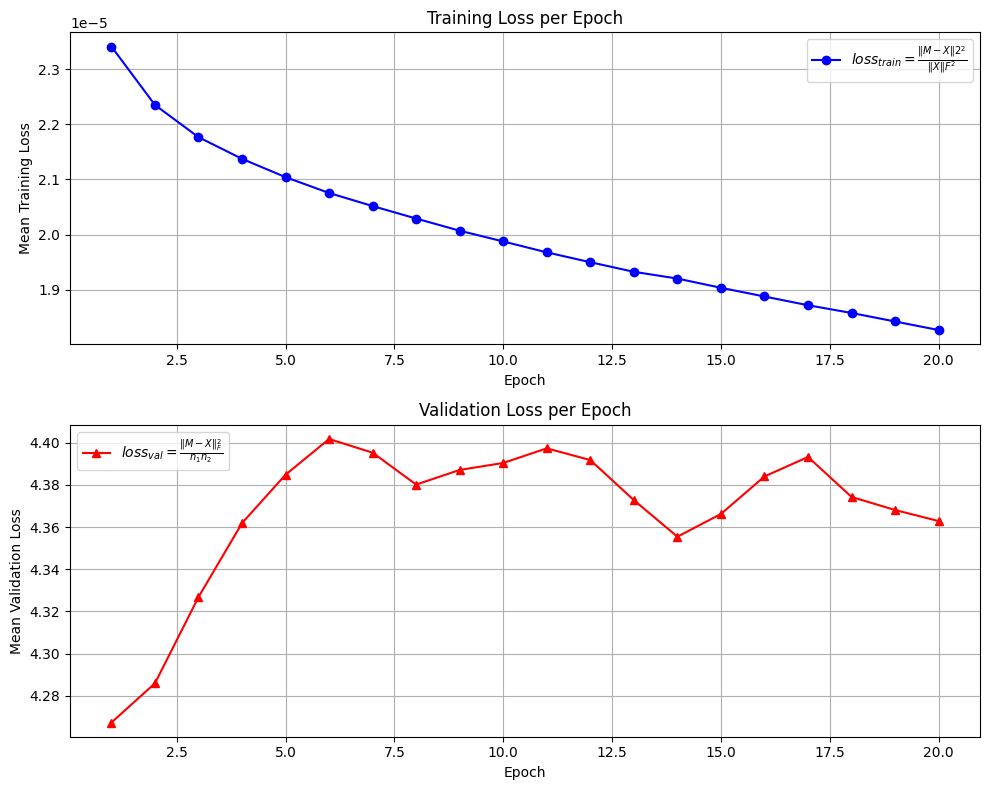
\includegraphics[width=\textwidth]{output_30_06}
    \caption{Training and validation loss for 30\% sampling rate and 6 SNR}
    \label{fig:output_30_06}
\end{figure}

\begin{figure}[htbp]
    \centering
    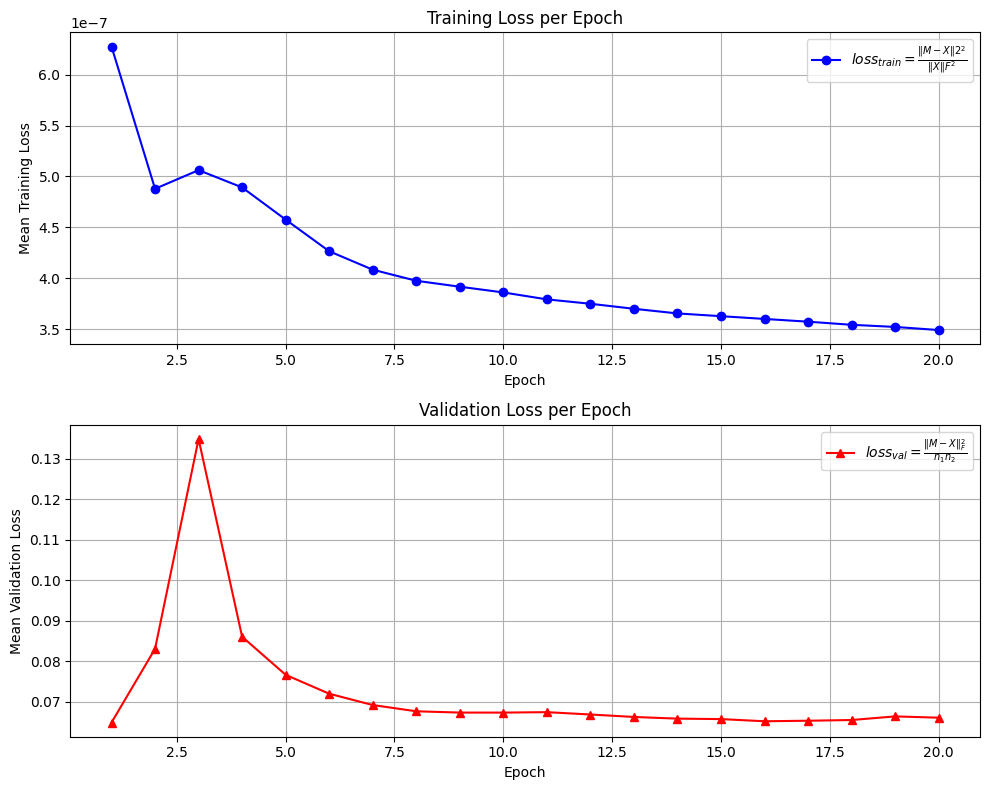
\includegraphics[width=\textwidth]{output_80_05}
    \caption{Training and validation loss for 80\% sampling rate and 5 SNR}
    \label{fig:output_80_05}
\end{figure}

\begin{figure}[htbp]
    \centering
    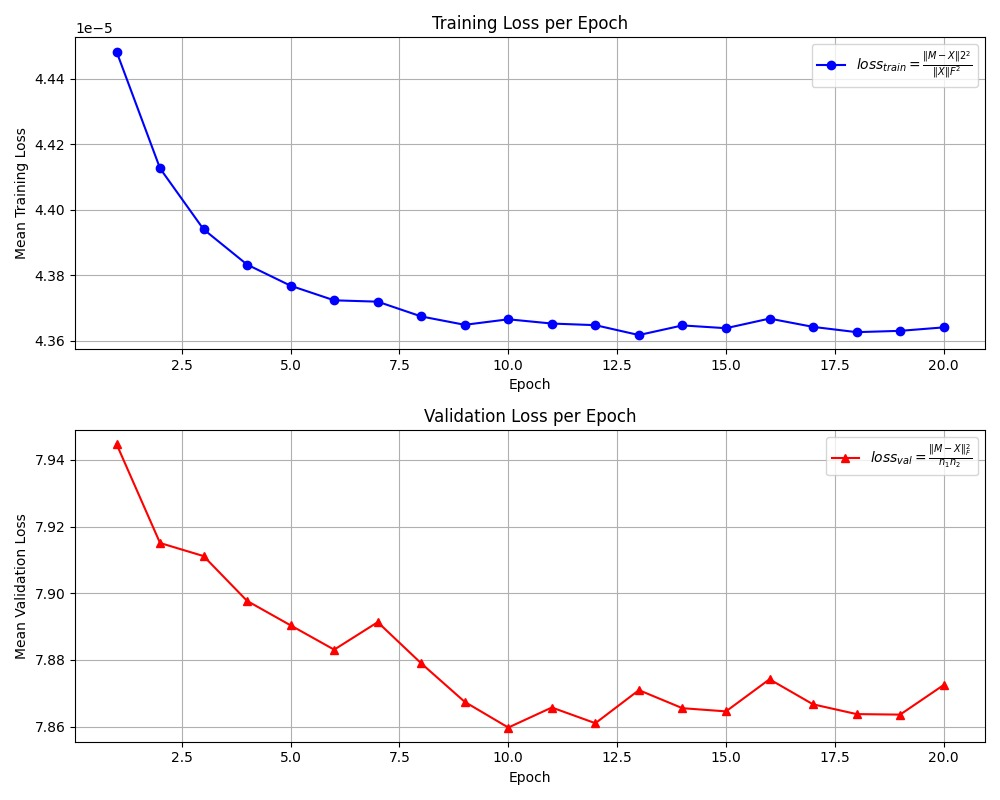
\includegraphics[width=\textwidth]{output_20_03}
    \caption{Training and validation loss for 20\% sampling rate and 3 SNR}
    \label{fig:output_20_03}
\end{figure}

\begin{figure}[htbp]
    \centering
    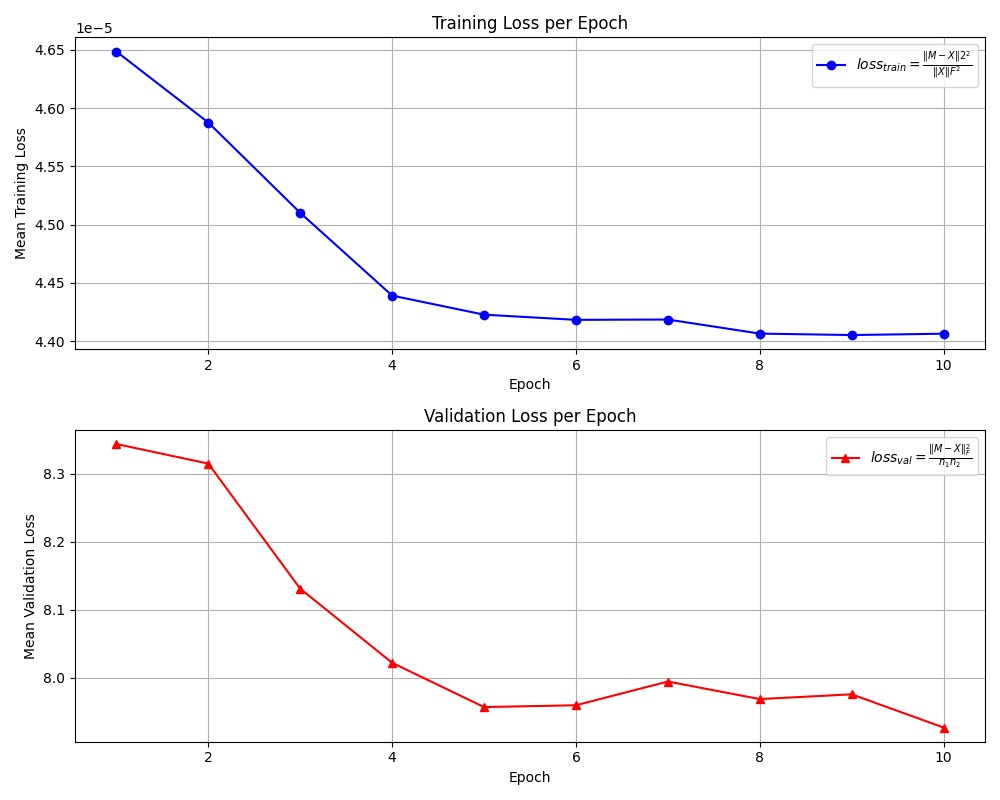
\includegraphics[width=\textwidth]{output_80_09}
    \caption{Training and validation loss for 80\% sampling rate and 9 SNR}
    \label{fig:output_80_09}
\end{figure}

Given this inherent unpredictability of ConvHuberMC-Net, we decided to exclude it from further analyses (on image inpainting and on matrices of shape (400 \(\times\) 500)) until we can pin the issue down. Our hypothesis is that the issue is related to the smooth and convex nature of matrix factorization algorithms and their operations and how they might not, therefore, be the optimal kind of algorithms for deep unfolding, unlike algorithms involving non-smooth operations, e.g., ALM. This also explains the fact that rarely anyone has unfolded algorithms involving matrix factorization so far. Before shelving the model, we did attempt to address the uncertainty in performance by learning the pseudoinverse that appears in Huber regression. However, this led to even more problematic performance, as now the model became completely insensitive to changes in sampling rate and SNR. For example, the two extreme combinations of 20\% sampling rate and 3 SNR and 80\% sampling rate with 9 SNR have nearly identical ranges for the training and validation losses, as shown in Figure \ref{fig:output_20_03} and Figure \ref{fig:output_80_09}. We ultimately dismissed this idea and, though we have shared a case of ConvHuberMC-Net outperforming the rest of the algorithms, it should be noted that this is not the case for all cases.

% When you are done with these 4 graphs, come to the fact that although our model especially HuberMC is sus at some times (for e.g share its loss patterns for 30% (DB 6 - ve light) sampling rate - up and down val loss), but at other times it has also performed normally. Here you can share its performance at (80% with 5 DB +ve light) sampling where the loss is decreasing with increase in DB generally speaking. Intepret both cases. Conclude this section by saying that due to the unpredictability and unsatisfactory performance of hubermc we choose not to go ahead with it while doing experimentation on image inpainting. Maybe link the reason of its sus performance to the nature of matrix factorization algorithms which are smooth and convex most of the time and hence the DNN might have some troubles in terms in learning when it comes to smooth operations such as found in matrix factorization as compared to non-smooth operations found in ALM type approaches.
% Considering these sus cases, we also considered learning the psuedoinverse as well however for some reason (if you can come up with some to likh dena) the loss trajectories became indifferent to the sampling and db combination and for each combo the val loss was in between 7 and 8. Here show the pic/graphs at 80% 9DB vs 20% 3DB and show both are in similar ranges in terms of val loss. Hence we dismissed this idea. Hence although at first it seems like it has performed way better for the 20% case, its not following the expected pattern for other combos. We finish HuberMC here. 
% ConvMC on the other hand has shown tremendous results beating many of the algorithms in synthetic 150 x 300, hence we go ahead and test it with all other algorithms in image inpainting. Suprisingly, we observed that although we did not take into account sort of noise in the $L$ update or neither the lagrange multiplier update, it still was able to after training on white-noise and GMM noise perform exceedingly well. This may prove our previous hypothesis where we claimed that the 'learning' feature of DNN might still be able to handle 'seeimgly' out - of - distribution tasks.
% Before ending the discussion on the first graph comment how the seemingly state of the art method L0-BCD has not performed to its expectations and other algorithms such as M-est are beating it. This suggests that these methods are signficantly related with the matrix dimension size with no general trend. This will be proven later in the next graph when we show the results for 400 x 500 synthetic. 
% For 400 x 500 synthetic just go ahead and intepret the results as they are but dont forget to mention how the above results where L0-BCD was not performing relatively better than M-est now its 10x better. Breifly mention again how we skipped hubermc in this graph due to its unpredictable and unsatisfactory performance. Share only one case of 20% and 3DB where the val loss is increasing but train loss is decreasing. 
The case for matrices of shape (400 \(\times\) 500) is shown in Figure \ref{fig:mse_snr_400_500}. It is obvious that merely changing the shape of matrices involved in the optimization process resulted in noticeable changes. \(\ell_0\)-BCD, which was far from the top, now outperforms every other algorithm by a big margin. It is uniformly followed by M-estimation, \(\ell_p\)-reg, \(\ell_p\)-ADMM, ORMC, and ConvMC-Net. This small yet important finding regarding the significance of matrix shape in matrix completion problems also requires further investigation.

After the detailed experimentation on synthetic dataset, we transitioned to image inpainting. The results for both $150 \times 300$ and $400 \times 500$ are summarized in Table \ref{tab:psnr_ssim_150_300} and \ref{tab:psnr_ssim_400_500}. From Table \ref{tab:psnr_ssim_150_300} we observe that surprisingly $\ell_{p}$-reg takes the lead in almost all of the combinations with second place going to either $\ell_{0}$-BCD or M-Estimation. This might suggest that the parameters such as $\sigma$ required for $\ell_{0}$-BCD algorithm i.e. which controls the outlier presence in the matrix needs to be fine-tuned because its very unlikely it performs not the best among all others considering its complete dominance in for the matrix size $400 \times 500$ as shown in \ref{tab:psnr_ssim_400_500}. Furthermore, if we start to take into account the inference times of each of these methods, $\ell_{0}$-BCD and M-estimation are at the top with $\ell_{p}$-reg or $\ell_{p}$-ADMM taking nearly $100\times$ of the time to achieve similar performance for or lower performance in the case of $\ell_{p}$-ADMM. 

We also observe regarding our proposed model, ConvMC-Net a poor performance in all combinations despite its seemingly overwhelming inference time. This can be attributed to the fact that we discussed in detail in Section 2 and 3 that such PCP methods aren not flexible to deal with impulsive noises, even more so if the objective function does not incorporate even white noise. However, we do observe of what one can deem to be anomaly at Image 8 of $150 \times 300$ dimensions. The PSNR is almost in the range of $40$'s and SSIM is nearly $0.9$ something which is way greater than the rest of the values. 

However, to test whether this was indeed an anomaly, we look at the below Table \ref{tab:psnr-ssim} which shows only ConvMC-Net's result for sampling rate $20\%$ and DB as %5.0%
\begin{table}[h]
\centering
\begin{tabular}{|c|c|c|}
\hline
\text{Image} & \text{PSNR} & \text{SSIM} \\
\hline
1 & 32.98 & 0.57 \\
2 & 33.41 & 0.61 \\
3 & 32.83 & 0.52 \\
4 & 33.40 & 0.58 \\
5 & 33.50 & 0.60 \\
6 & 33.96 & 0.63 \\
7 & 33.53 & 0.59 \\
8 & 34.75 & 0.63 \\
\hline
\end{tabular}
\caption{PSNR and SSIM values for ConvMC-Net with 20\% sampling rate and DB 5.0}
\label{tab:psnr-ssim}
\end{table}
As if this is not surprising enough, we observe similar results in most of the combinations even for the case of $400 \times 500$. This result, we believe is still not to be taken as completely trustworthy and requires further investigation. This is because, if the same model does not perform even close to other algorithms in the synthetic dataset, it should be very unlikely it overwhelms for the case of image inpainting experimentation.
% Note: For the image inpainting intepretation, use the current combo in the table i.e. 5DB and 50% sampling rate and attach convmc  results to the table for both 150 x 300 and 400 x 500. Here comment how seemingly convmc is performing way worse than other algorithms but somehow (if you can come up with any scientific reason then use it) for other combos its is dominating all other algorithms with PSNR in ranges of 35 - 45 and ssim in ranges of 0.8-0.95 etc. (You can even show a small table for it as well.) And comment on the L-BCD performance difference between 150 x 300 and 400 x 500 similar to the synthetic one. But an additonal suprise here is that lp-reg is dominating the 150 x 300 section and its in close second for 400 x 500 even beating M-estimation is some combos which was not the case for synthetic. % Experiment 1

 % Chapter 3

\chapter{Discussion, Future Prospects, and Reflections} % Write in your own chapter title
\label{Chapter5}
\lhead{} % Write in your own chapter title to set the page header

\section{Discussion and Future Prospects} % will change this name 
% Limitations + the fact that experimentation is ongoing not perfect but still has future prospect. May also mention in which types of data (image vs synthetic or 150 x 300 vs 400 x 500)  what algorithms of ours performed best. And what could have been done better overall (borrow content from section 5 and 6). Bonus section perhaps on our RNN idea.
From our current results, we conclude that, on average, [blank] outperformed [blank] in [blank] task on a data set of size [blank]. And so on...

Though we do not yet have conclusive results, our models clearly are not performing consistently. We know from domain knowledge that a higher sampling rate, SNR, or both should lead to a lower loss, higher PSNR, and higher SSIM. However, this expectation has not been met and this is perhaps the biggest problem of our models. Therefore, experimentation is as yet ongoing with the hope that we figure out whether the problem is due to suboptimal hyperparameters, an issue of model implementation, or the underlying iterative algorithm's inherent inability to be effectively unfolded. Once we discover the root cause, it would become much easier to improve our results and demonstrate that deep unfolding is a viable approach for matrix completion problems and that it can work with a number of different iterative algorithms. In the case that we fail to demonstrate this, future works might look into the possibility of radically different approaches, such as recurrent neural networks or methods from the expanding field of generative AI.

\section{Reflections}
The project provided profound insights into the challenges and complexities of unfolding algorithms for matrix completion in noisy environments. In hindsight, despite the fact that this was an entirely new area for us, a few missteps costed us a lot of valuable time and slowed our progress. For example, upon realizing that ConvMC-Net cannot be fairly compared with ADMM-Net due to difference in model assumptions, it might have been better to consult our peers about whether this is really the case, and, if it is, can we somehow modify ConvMC-Net instead of jumping to a new algorithm. Similarly, When we decided to unfold M-estimation, we could have asked whether some other algorithm would be more friendly to deep unfolding (as we primarily chose M-estimation based on the closeness of its results to those of $\ell_0$-BCD). These lessons will hopefully guide us in our future projects. % Experiment 2

%\input{./Chapters/Chapter6} % Results and Discussion

%\input{./Chapters/Chapter7} % Conclusion

%% ----------------------------------------------------------------
\label{References}
\lhead{}  % Change the left side page header to "References"
\renewcommand\bibname{References}
\bibliographystyle{IEEEtran}  % Use "unsrtnat" BibTeX style for formatting the references

\bibliography{references}  % The references information are stored in the file named "references.bib"
\begin{comment}
%% ----------------------------------------------------------------
\setstretch{1.3}  % It is better to have smaller font and larger line spacing than the other way round

% Define the page headers using the FancyHdr package and set up for one-sided printing
\fancyhead{}  % Clears all page headers and footers
\rhead{\thepage}  % Sets the right side header to show the page number
\lhead{}  % Clears the left side page header

\pagestyle{fancy}  % Finally, use the "fancy" page style to implement the FancyHdr headers


%% Select only one of the certification pages  
%\CertificationMSc{}
\CertificationBSc{}
\clearpage  % Certification ended, now start a new page


%% ----------------------------------------------------------------
% End of the pre-able, contents and lists of things
% Begin the Dedication page
\setstretch{1.3}  % Return the line spacing back to 1.3
\pagestyle{empty}  % Page style needs to be empty for this page
\dedicatory{For/Dedicated to/To my\ldots}


%% ----------------------------------------------------------------
\pagestyle{fancy}  %The page style headers have been "empty" all this time, now use the "fancy" headers as defined before to bring them back

%% ----------------------------------------------------------------
\setstretch{1.5}  % Set the line spacing to 1.5, this makes the following tables easier to read
\clearpage  % Start a new page
\lhead{\emph{Abbreviations}}  % Set the left side page header to "Abbreviations"
\listofsymbols{ll}  % Include a list of Abbreviations (a table of two columns)
{
% \textbf{Acronym} & \textbf{W}hat (it) \textbf{S}tands \textbf{F}or \\
\textbf{LAH} & \textbf{L}ist \textbf{A}bbreviations \textbf{H}ere \\
}

%% ----------------------------------------------------------------
% Now begin the Appendices, including them as separate files

\addtocontents{toc}{\vspace{2em}} % Add a gap in the Contents, for aesthetics

\appendix % Cue to tell LaTeX that the following 'chapters' are Appendices

\input{./Chapters/AppendixA}	% Appendix Title

%\input{./Chapters/AppendixB} % Appendix Title

%\input{./Chapters/AppendixC} % Appendix Title

\addtocontents{toc}{\vspace{2em}}  % Add a gap in the Contents, for aesthetics
\backmatter

\end{comment}
\end{document}  % The End
%% ----------------------------------------------------------------
